% CHAPTER - Design ---------------
\chapter{Design}%
\label{ch:design}
In the design phase, the solution is developed in the various domains and a
thorough specification is written, paving the way for implementation. In this
chapter is presented the design for the various domains and subsystems identified.

\section{Navigation Virtual Subsystem}%
\label{sec:navig-virt-subsyst-design}
The Navigation subsystem hosts the core of the system functionality-wise, which is the control routine. This means that it should strive to not only make accurate readings and calculations but also be as efficient as possible in managing those processes in order to introduce very little delay and meet timing requirements. 

To meet these requirements as best as possible it should be capable of :

\begin{itemize}
    \item Gathering information from the physical domain at equally distant instants $kT_s$ and output an electrical representation of the command variable at equally distant instants $kT_o$;
    \item Acquiring commands from the Smartphone and Remote Vision Subsystems, identifying matches that will allow it to validate those commands and feeding them into the control rule in a useful format;
    \item Providing real-time feedback to the user about its status.
\end{itemize}


The first task should be idealizing the control system itself, understanding what inputs are needed to control the machine and then how it could be used to manipulate the wheels of the car. After that, the rest of system should be designed to fit the needs of the control rules and algorithms and use them to react as fast and consistently as possible within its own constraints and those of the other subsystems.
%
\subsection{Control}%
\label{sec:control-design}
The objective of the control module is to be capable of, with an input reference velocity and steering angle, outputting the appropriate command variables to achieve said references. The first step in its design is to conceptualize the car's model; since the interest lies in the motion of the car, the kinematic model will be the one to be studied.
\subsubsection{Conception Of Car Model}
\label{sec:concep}

\begin{figure}[!htbp]
\centering
       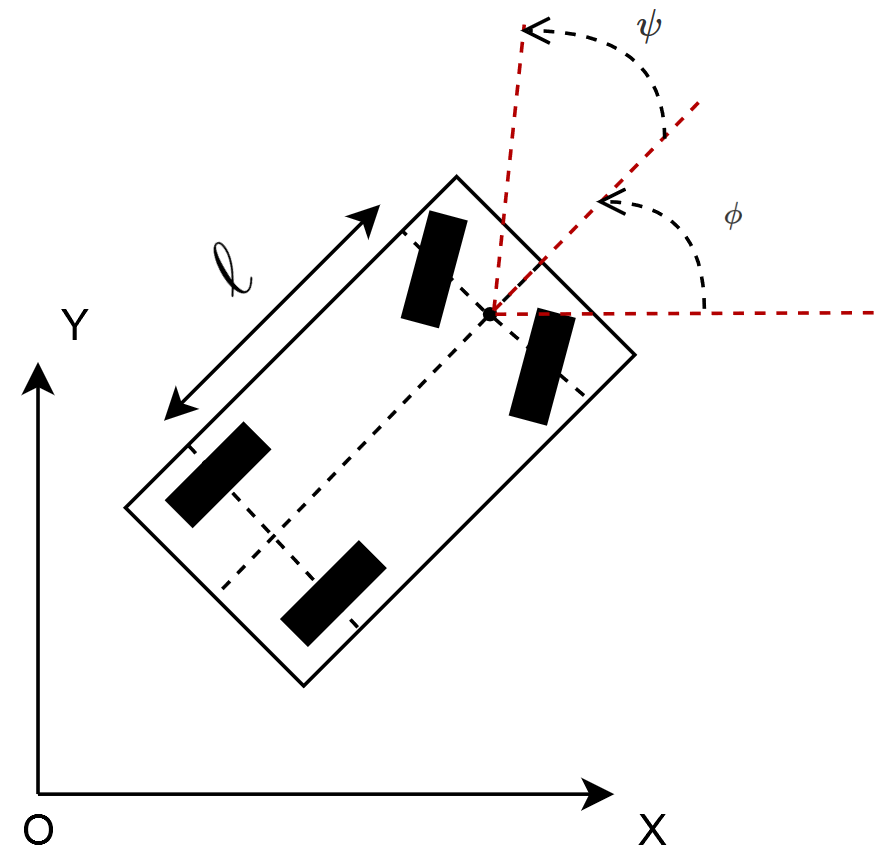
\includegraphics[page=1,width=0.6\textwidth]{img/kinematicModel.png} 
\caption{Kinematic Model of Car}
\label{fig:kinModel}
\end{figure}

Considering the kinematic model of a four-wheel vehicle with a wheelbase length $\ell$, a linear velocity v(t) and an angular velocity $\omega(t)$ the following situation will occur: since the rear wheels will remain in the same position no matter where the car is facing towards, they will be facing whatever orientation, $\phi$, the car is facing, however, in order for the car to be capable of moving into wherever the user tells it to, the front wheels must turn, ergo a steering angle $\psi$, must be considered. The resulting direction the car will be going in is $\phi + \psi$. With these considerations, a desired angle of tilt $\theta$ and considering that $\phi=0$, in other words, that whatever direction the car is told to face, it will be relative to its current direction, the following model is obtained:
\begin{align}
\dot{x}&=v(t) cos(\psi)\\
\dot{y}&=v(t) sin(\psi)\\
\dot{\psi}&=\omega(t)=\frac{v(t)}{\ell}\theta
\end{align}
However this model is not enough for simulation purposes. The simulation has the objective of granting the designers clear ideas of the response of the systems towards given inputs, therefore, for implementation purposes, the simulation must give feedback on the position of the car, its heading and the linear velocity of the right rear wheel ($v_r$), and the left rear wheel ($v_l$) therefore the model will have to changed with these details in mind, which can be achieved considering that:
\begin{align}
\omega(t)&=\frac{v_r(t)-v_l(t)}{\ell}\\
v(t)&=\frac{1}{2}(v_r(t)+v_l(t))
\end{align}
Solving the system above for $v_r$ and $v_l$:
\begin{align}
v_ r(t)&=v(t)+ \frac{\omega(t)\ell}{2}\\
v_l(t)&=v(t)-\frac{\omega(t)\ell}{2}
\end{align}
Returning the model in order to $\dot{x}$ and $ \dot{y}$:
\begin{align}
\dot{x}&=v(t) cos(\psi)-\frac{\ell}{2}\omega(t) sin(\psi)\\
\dot{y}&=v(t) sin(\psi)+\frac{\ell}{2}\omega(t) cos(\psi)\\
\dot{\psi}&=\omega(t)=\frac{v(t)}{\ell}\theta
\end{align}
\subsubsection{Simulation Model}
The mathematical model determined in Section~\ref{sec:concep} was simulated in
the Matlab/Simulink environment. Converting the mathematical model into a
simulink subsystem yields (Fig.~\ref{fig:carModel}):
\begin{figure}[!htbp]
\centering
       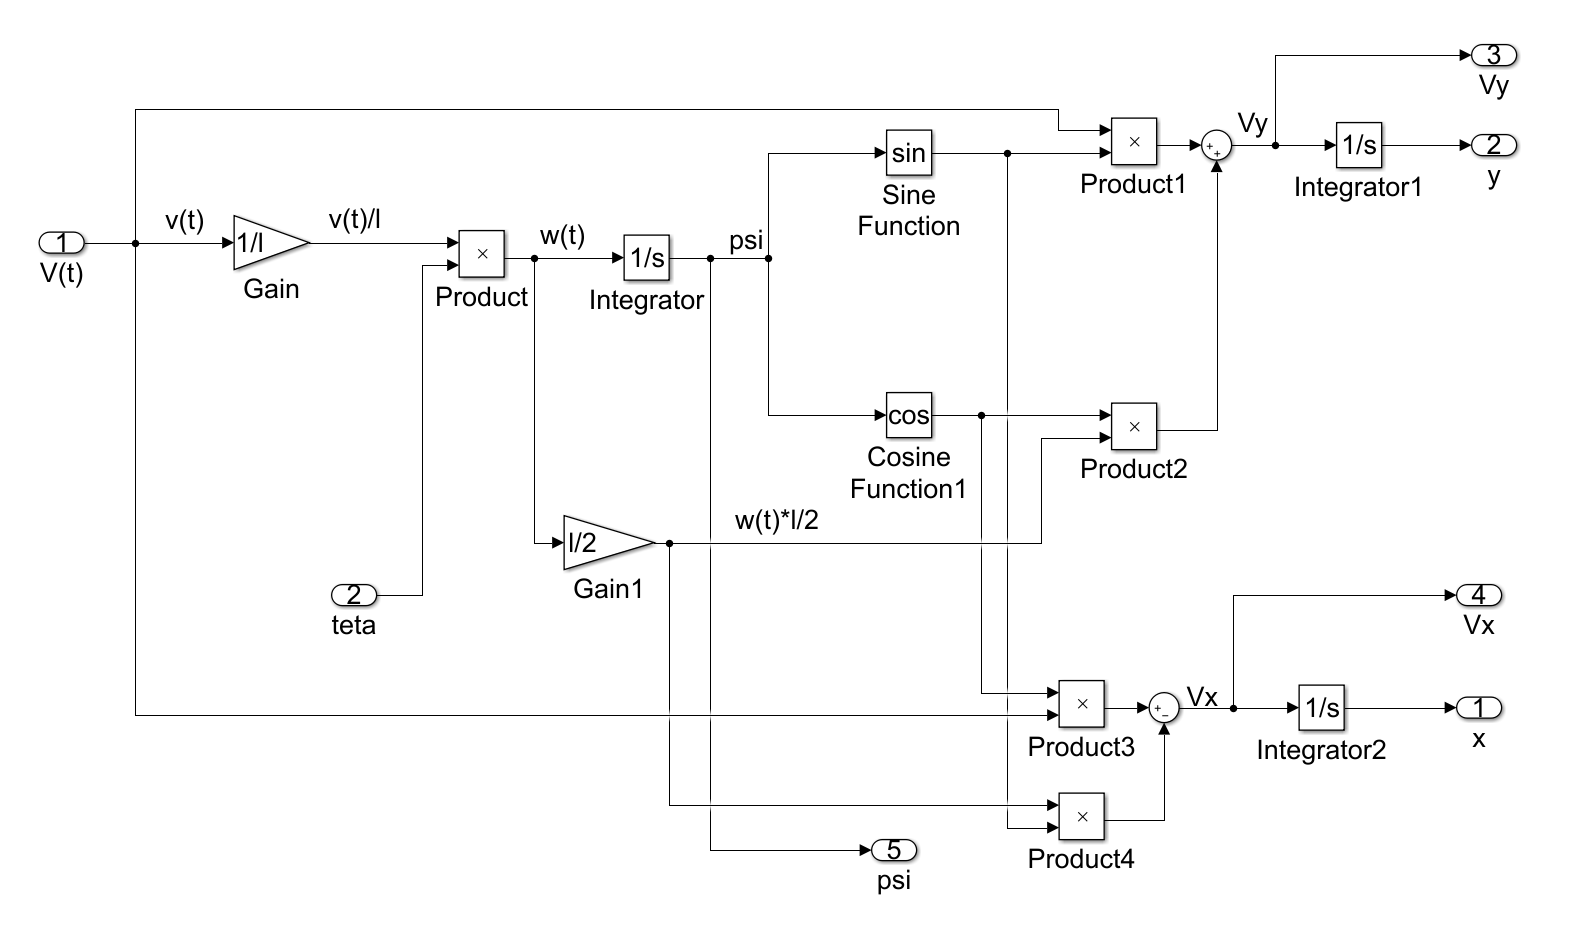
\includegraphics[page=1,width=1\textwidth]{img/subsystem.png} 
\caption{Car Model in a Simulink Subsystem}%
\label{fig:carModel}
\end{figure}
After obtaining the model of the car, the control simulations of the system may begin:
\begin{figure}[!htbp]
\centering
       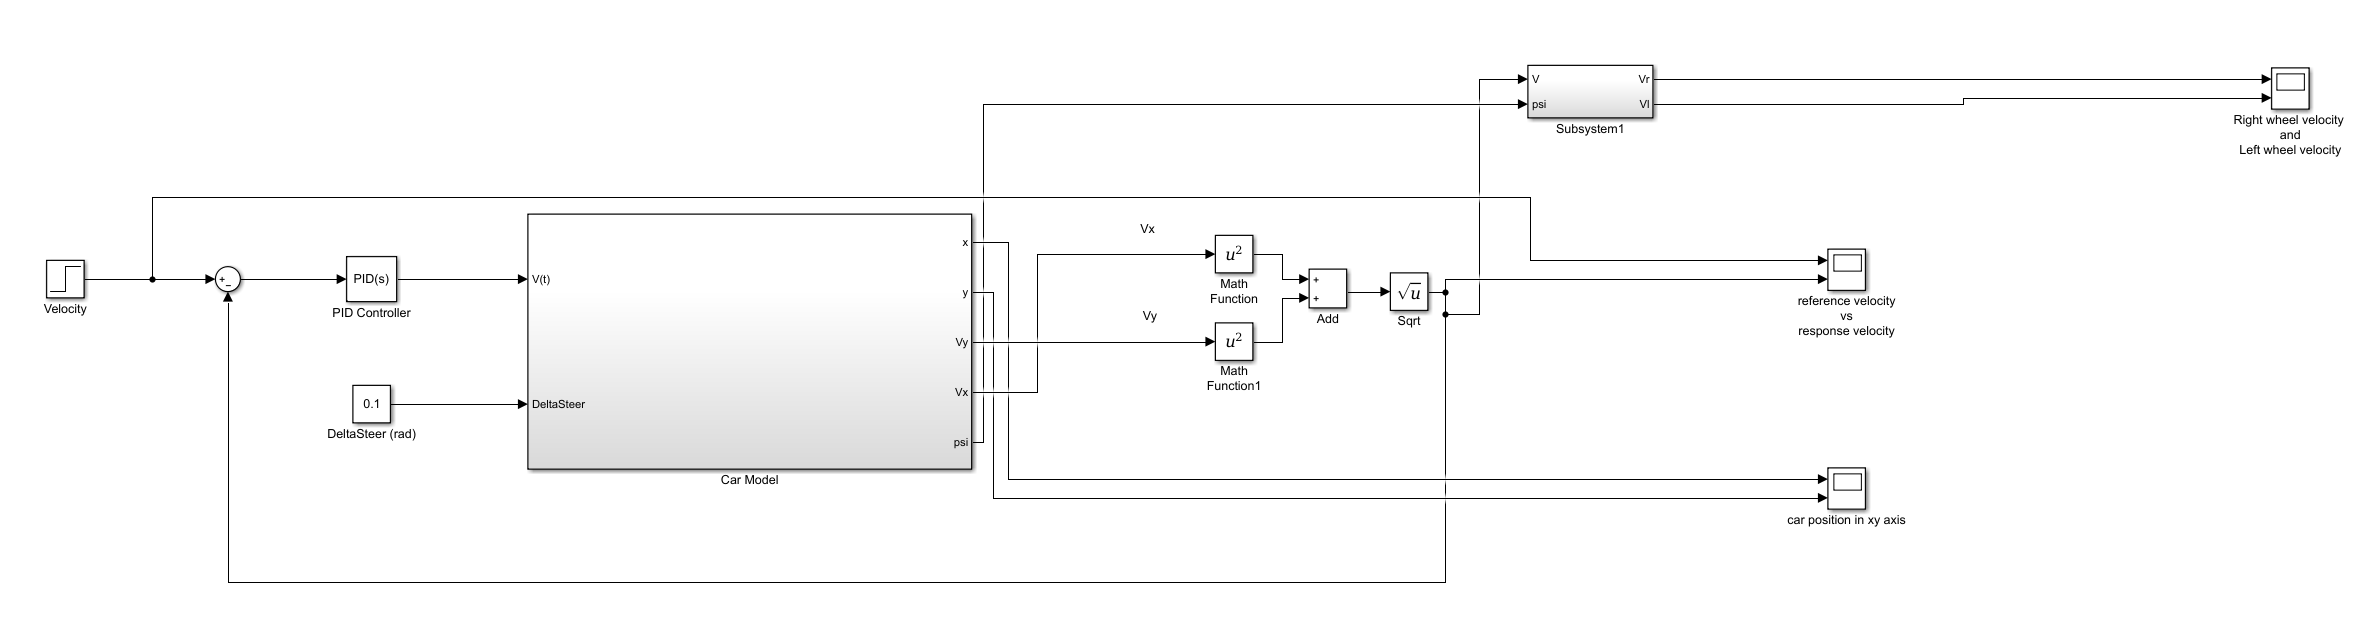
\includegraphics[page=1,width=1\textwidth]{img/system.png} 
\caption{Simulation Schematic}
\end{figure}\\
The simulation schematic uses the model in Fig.~\ref{fig:carModel} within the
`Car Model' subsystem to simulate the response of the system to a step reference
of the desired velocity and a constant reference of the angle to which the car
should turn towards. It calculates the norm of the velocity vector, returns it
as feedback and also uses it to pass through subsystem1 that will return the
different velocities at which each of the rear wheels must turn in order to
achieve said angle.
%%% Local Variables:
%%% mode: latex
%%% TeX-master: "../../../dissertation"
%%% End:

%SUBSECTION - control
\subsubsection{Optimal control parameters determination}
As the controller in use is a discrete PID, the first step is to find the optimal parameters.
For the first set of simulations, the aim is to find the values for the PID gains. As purpose of the car is to explore hazardous areas, the parameter Kd will be set as 0 due to the noise. 
For the first simulation, $K_d = 1$, $K_i = 1$, Linear speed = 1 m/s, $\theta =
0~\si{rad}$:
\begin{figure}[!h]
\centering
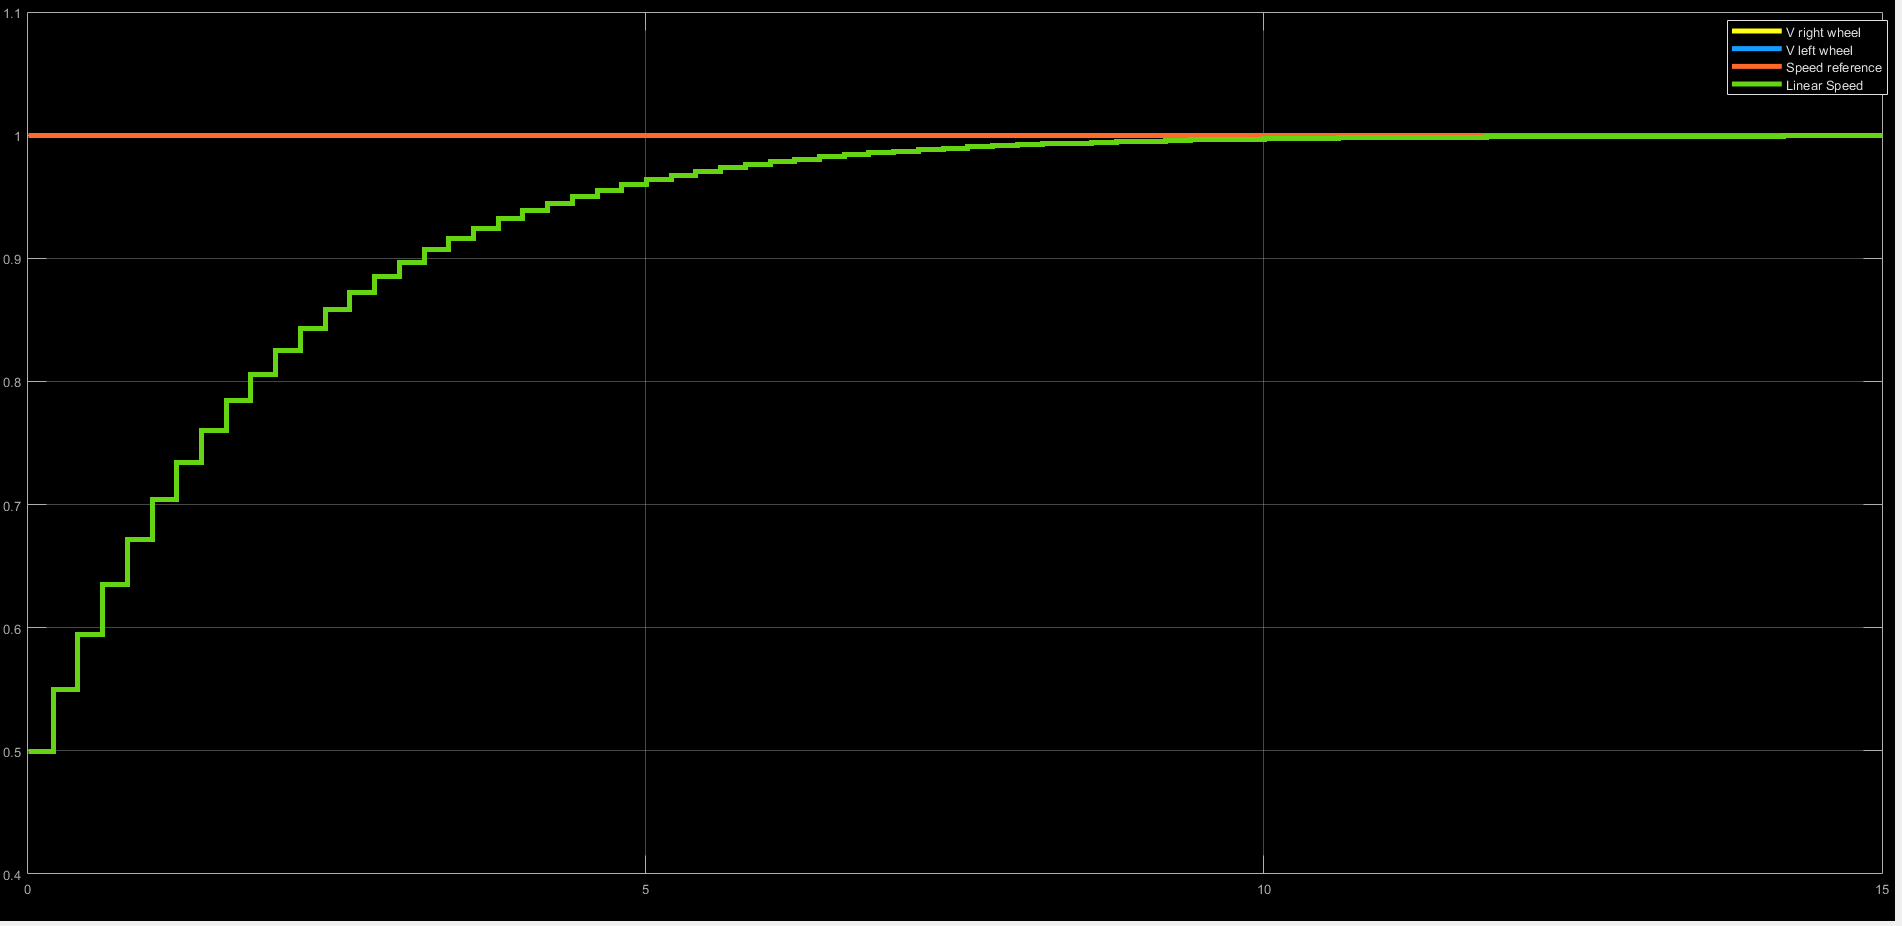
\includegraphics[width=1.0\textwidth]{./img/pid11.png}
\caption {\label{fig:pid1-p1i1}Kp=1, Ki=1}
\end{figure}
With this simulation, it is possible to see that the initial value of the velocity of the car is 0.5 m/s and it take about 7 seconds to reach steady state. 0.5m/s as an initial value for the linear velocity is a considerably high value and can cause the car to slide, therefore, the Kp value needs to get lower, for the initial value to get lower as well.
%\newpage
In this simulation, Kp will be set as 0.5 and Ki as 1.
\begin{figure}[!h]
\centering
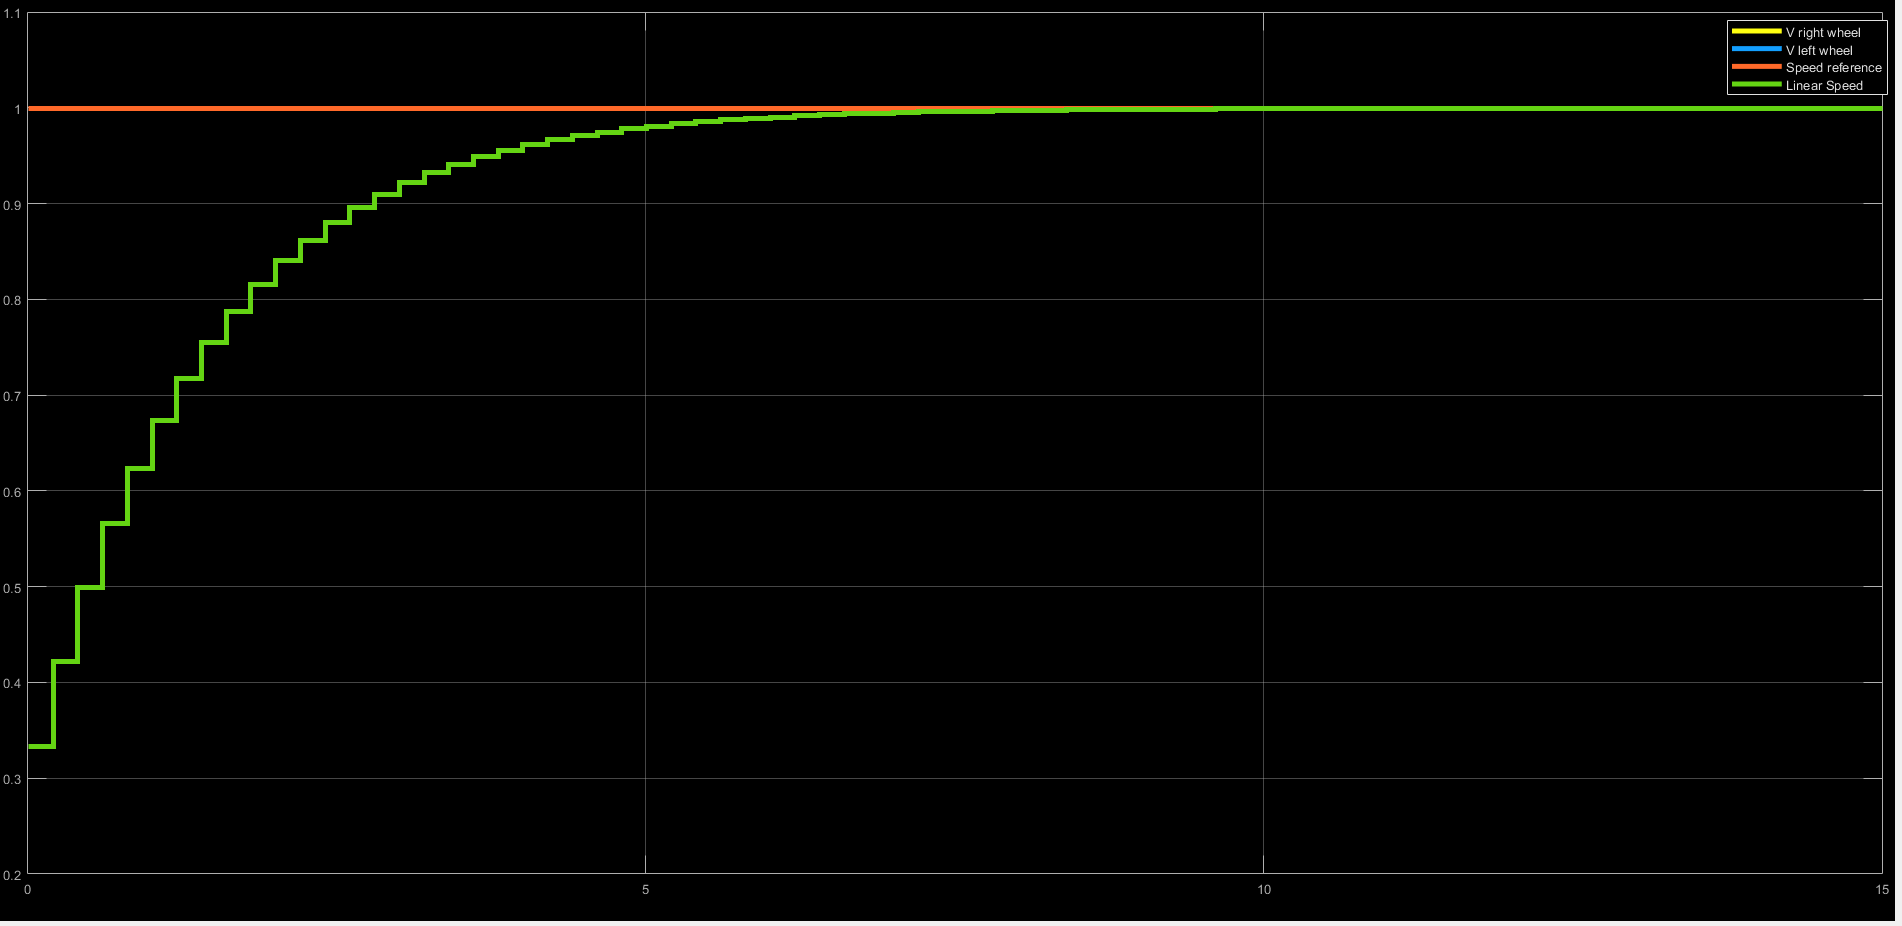
\includegraphics[width=1.0\textwidth]{./img/pid051.png}
\caption {\label{fig:pid1-p05i1}Kp=0.5, Ki=1}
\end{figure}
Changing the value of Kp to half of the initial value, it is possible to see that the initial linear speed is now 0.3 m/s, making it harder for the car to slide. It takes nearly 6 seconds for the car to reach steady state, thus the Ki value must be increased.
%\newpage
In this simulation, Kp will be set as 0.5 and Ki as 2.
\begin{figure}[!h]
\centering
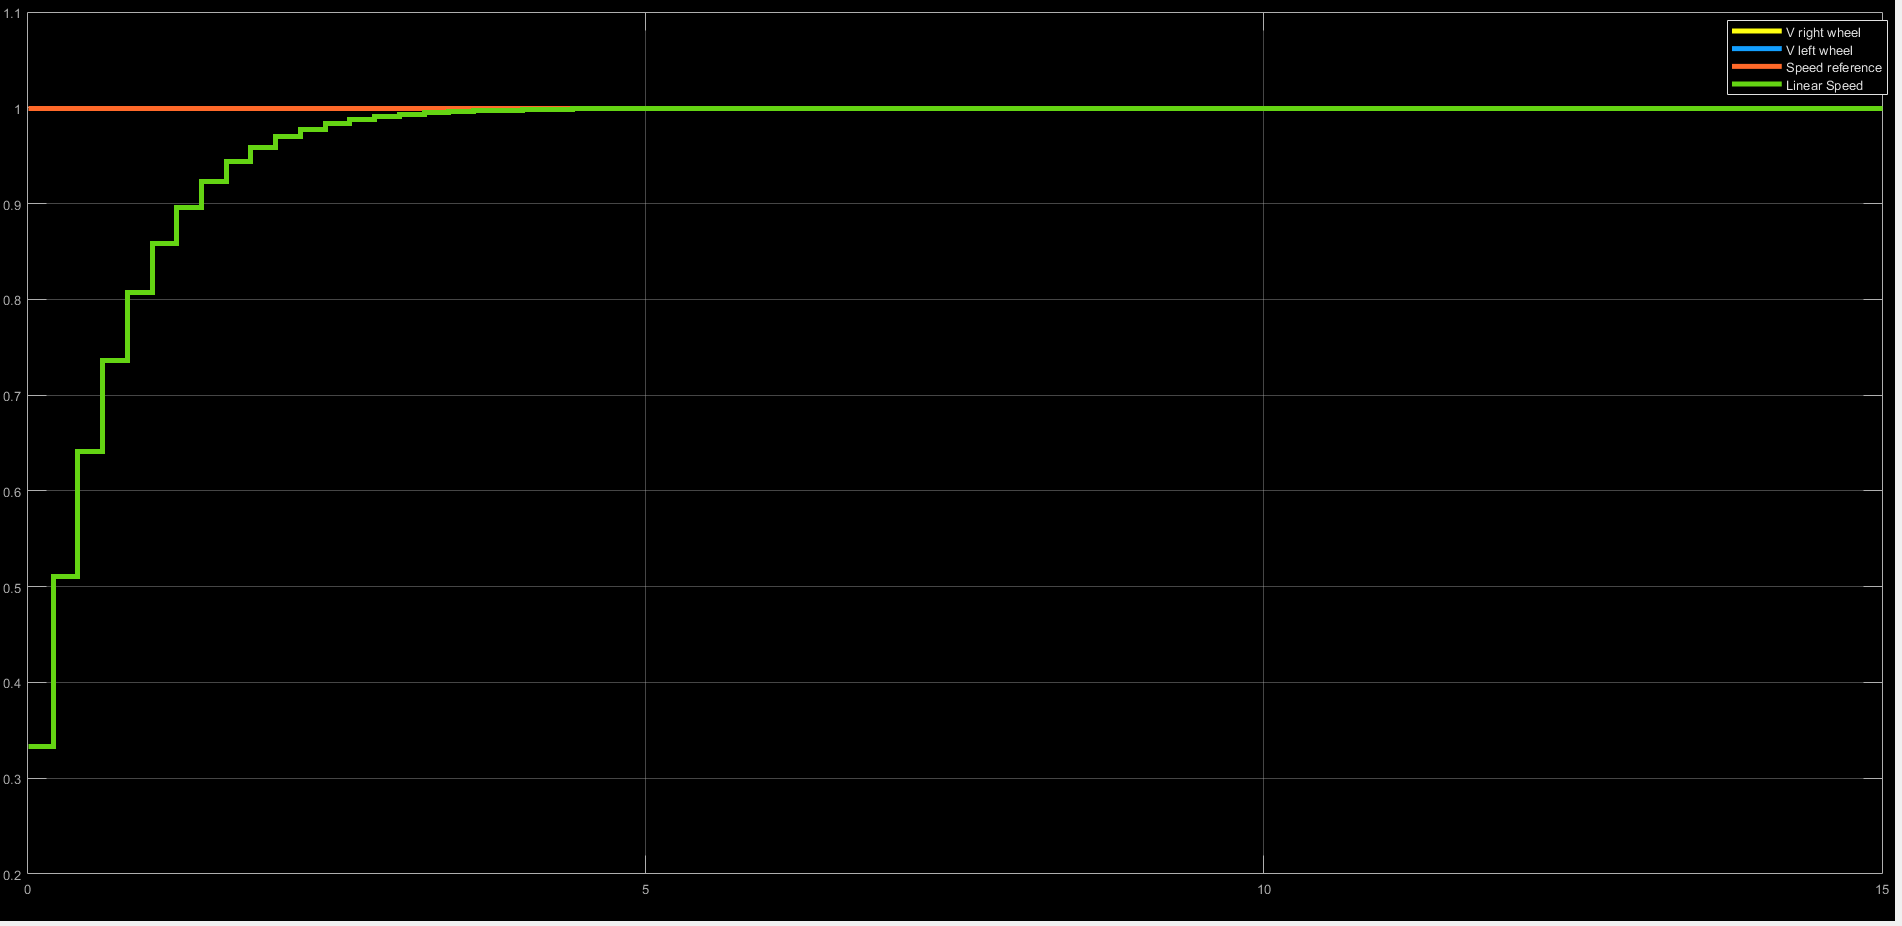
\includegraphics[width=1.0\textwidth]{./img/pid052.png}
\caption {\label{fig:pid1 - p05i2}Kp=0.5, Ki=2}
\end{figure}
As the Kp value was not changed, the initial linear speed value remains the same. As for the time it takes the car to reach steady state, it was reduced to 3 seconds due to the increase of the Ki parameter.\\
In ideal conditions, the aim would be for the car to reach the desired speed
instantly, but due to the real limitations, such as wheel sliding, 3 seconds is
a a safe value.
%
\subsubsection{Sample time determination}
In order to choose the sample time, one needs to take in consideration that with the decrease of the sample time, the processing overhead will increase and with the increase of the sample time, the system response will have abrupt changes affecting the performance of the car. So, in order to accommodate both necessities, the sample time will be set to 50ms.
%\newpage
\subsubsection{System response}
Having determined the parameters of the controller, the next step is to simulate the response of the system.
In order to predict the behavior of the car to a linear speed reference and angle of tilt (teta), some simulations were necessary. The output of the simulation is the plot of the linear speed of the car, the linear speed of both wheels (left and right) and the position of the car.
In order to plot the position of the car the Cartesian referential is used.\\
For the first simulation, the parameters were: Speed reference= 1m/s and teta=0 rad.\\
\begin{figure}[!h]
\centering
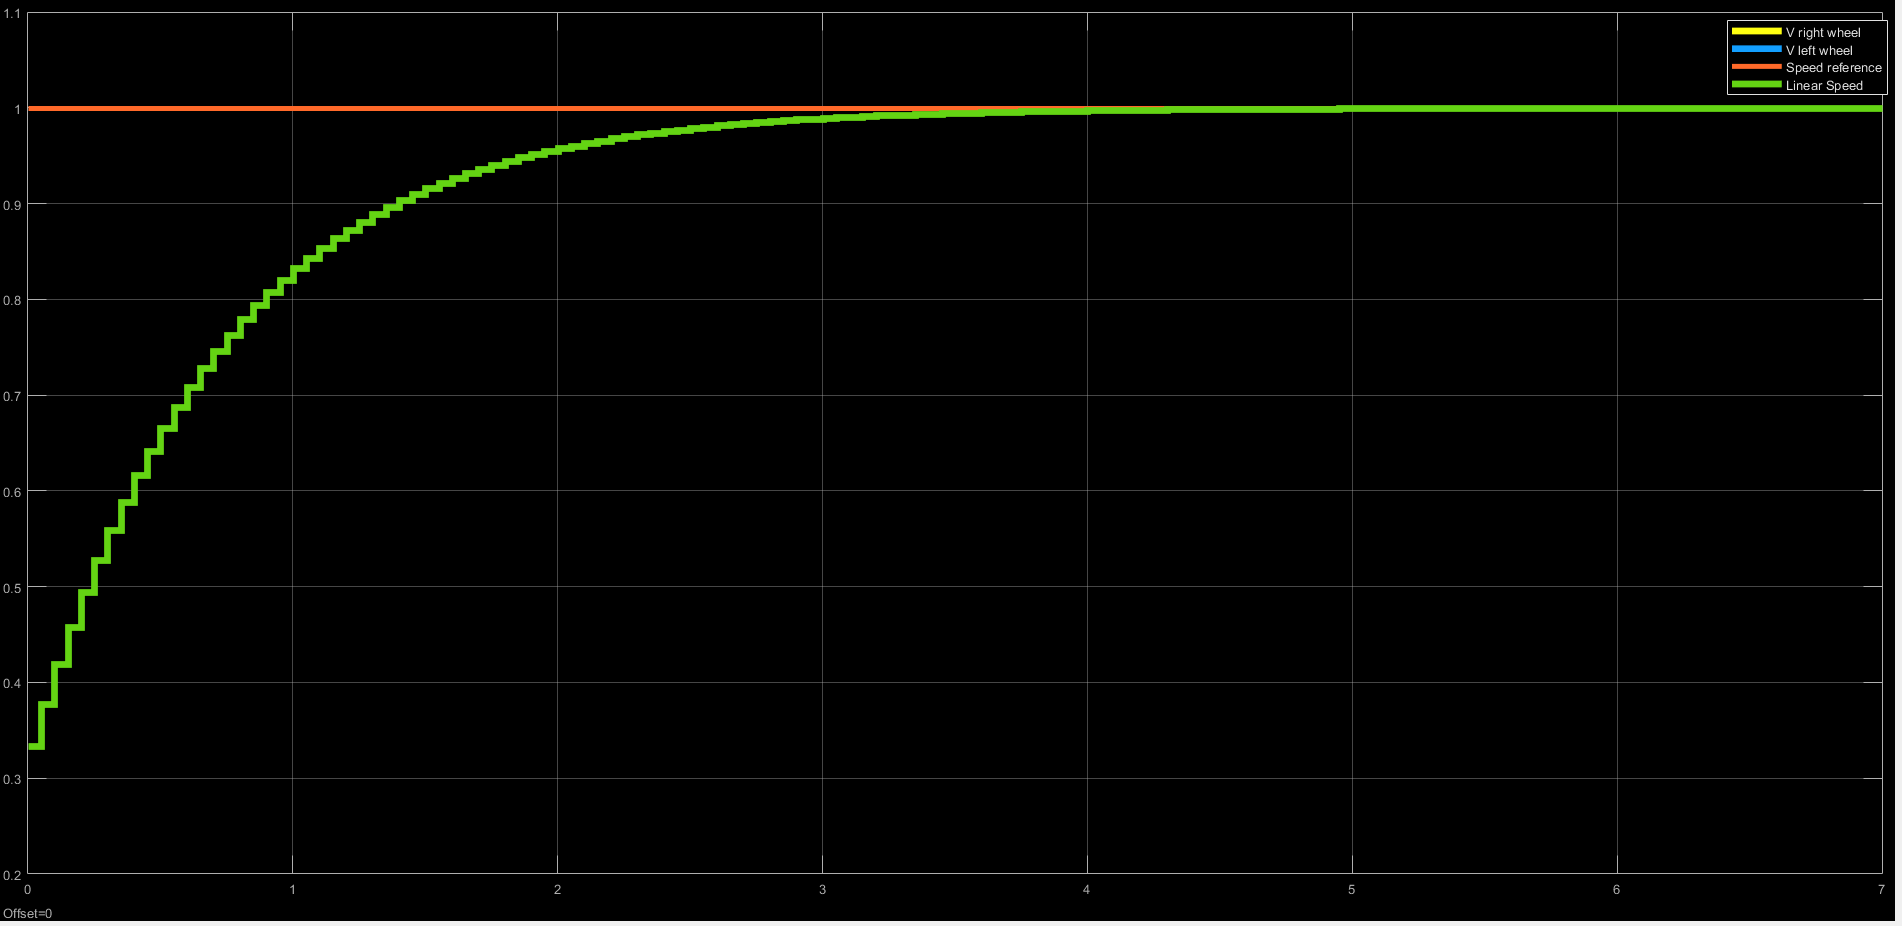
\includegraphics[width=1.0\textwidth]{./img/vel10.png}
\caption {\label{fig:sim1 - vel}Linear speed v=1m/s, teta=0rad}
\end{figure}
 As expected, the car linear velocity reached 1m/s. The angle of tilt is equal to 0 which means the car will be moving in a straight line, and as such, both wheels will are moving at the same speed of the car.\\
\newpage
\begin{figure}[!h]
\centering
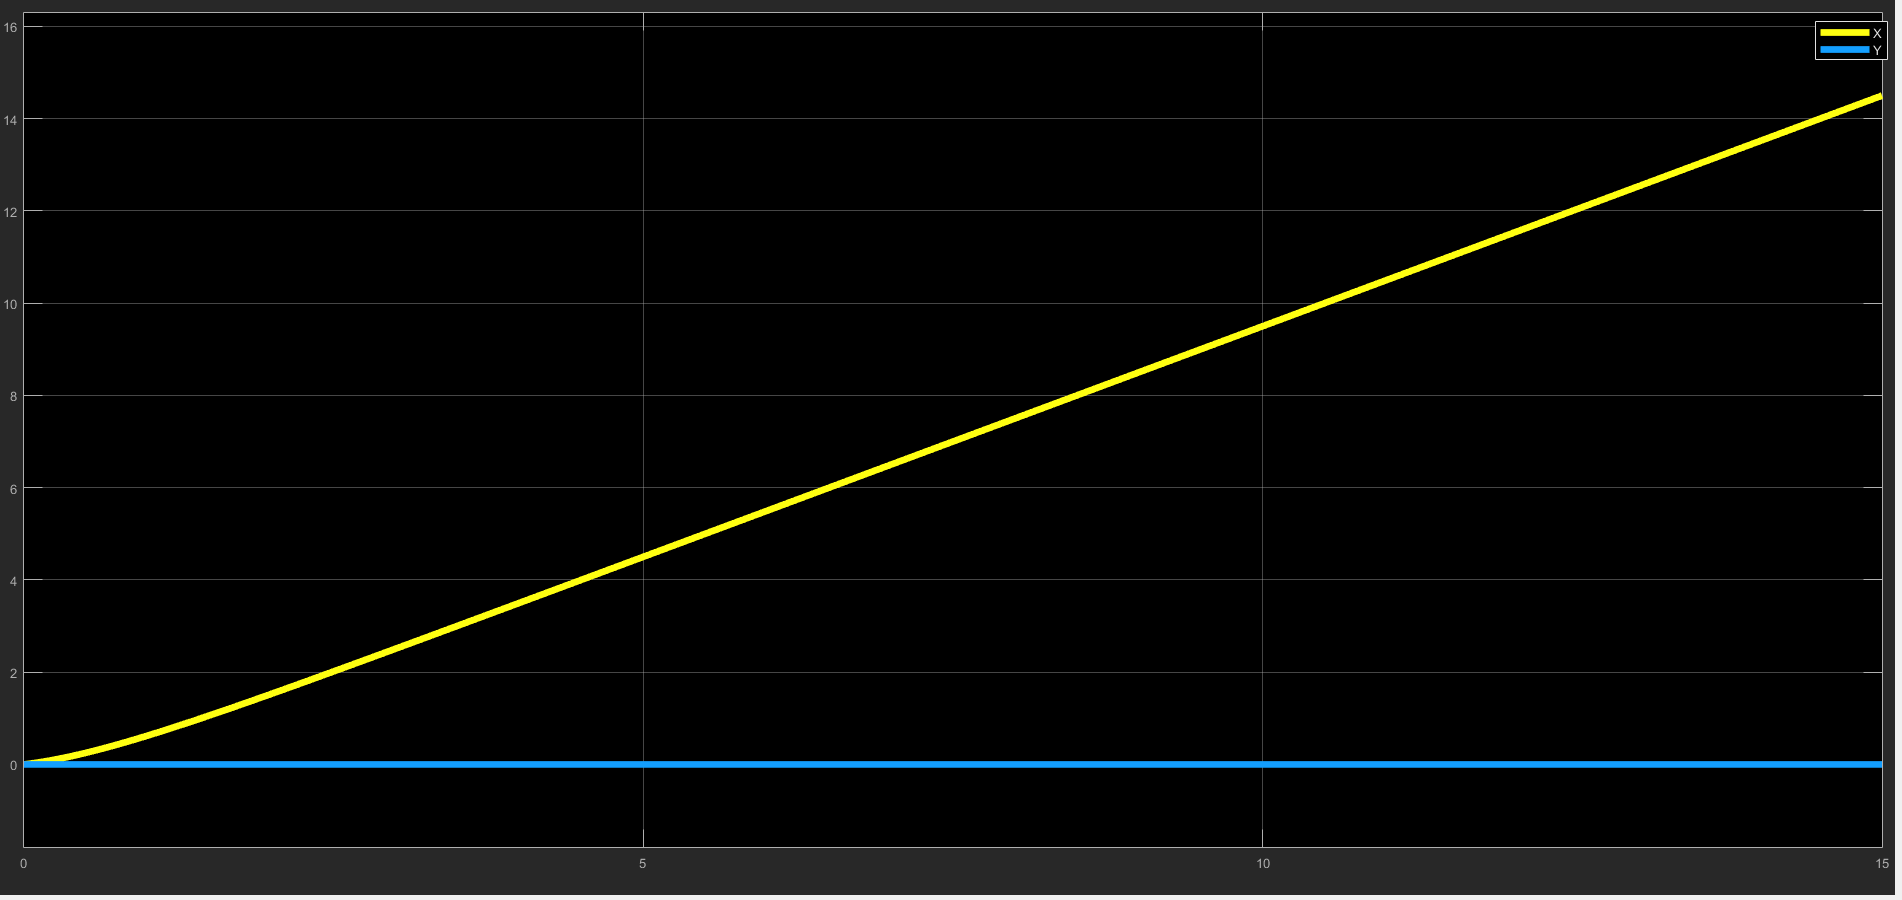
\includegraphics[width=1.0\textwidth]{./img/xy10.png}
\caption {\label{fig:sim1 - pos}Car position v=1m/s, teta=0rad}
\end{figure}
As the teta is equal to 0 rad, only 1 coordinate of the car is moving, as the figure \ref{fig:sim1 - pos} demonstrates. The x coordinate is equal to 0 the entire simulation time, and the y coordinate is increasing with a linear scope equal to the linear velocity of the car. This implies that the car is indeed moving in a straight line.\\
\newpage
Changing the teta to 0.1 rad to simulate constant tilt of the smart phone to the right, and maintaining the value of the speed reference in 1 m/s :\
\begin{figure}[!h]
\centering
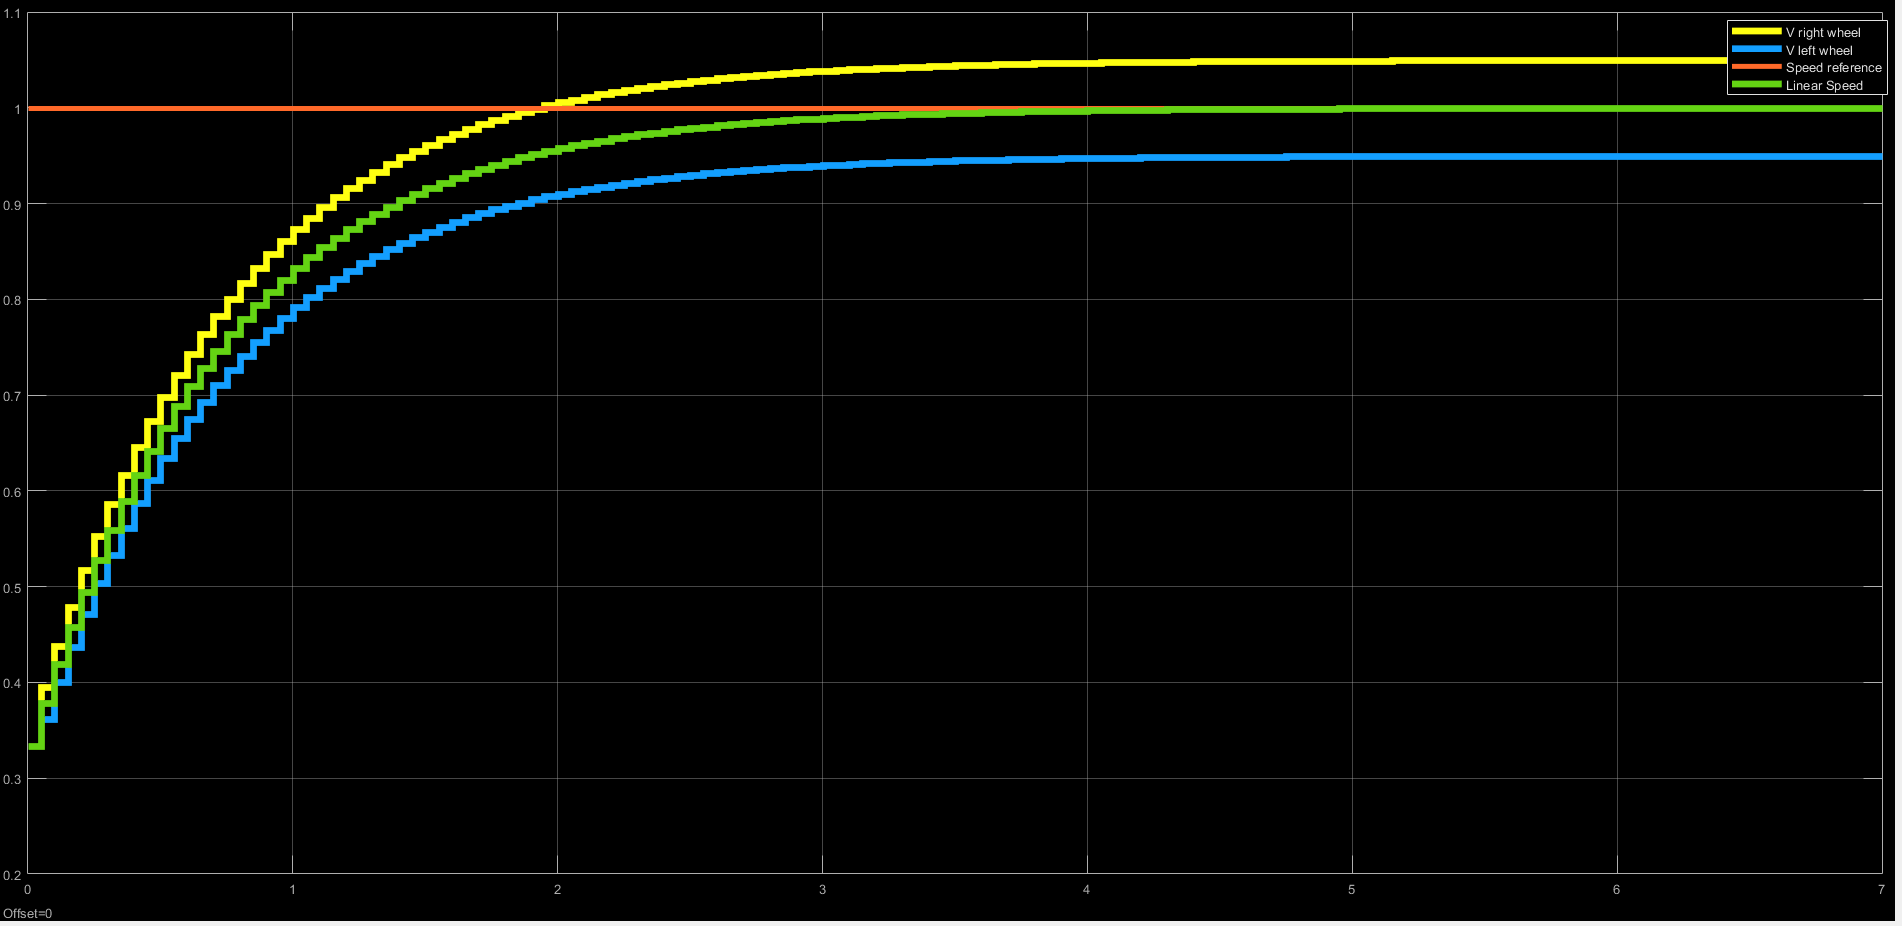
\includegraphics[width=1.0\textwidth]{./img/vel101.png}
\caption {\label{fig:sim2 - vel}Linear speed v=1m/s, teta=0.1rad}
\end{figure}
In this simulation it can be observed that having a angle of tilt not equal to 0, causes the left and right wheels to have different velocities, in order to make the car turn. Running more simulations with different values of teta, the outcome shows that the bigger the module of the value of teta, the bigger the difference between the linear velocities of the wheels.
\begin{figure}[!ht]
\centering
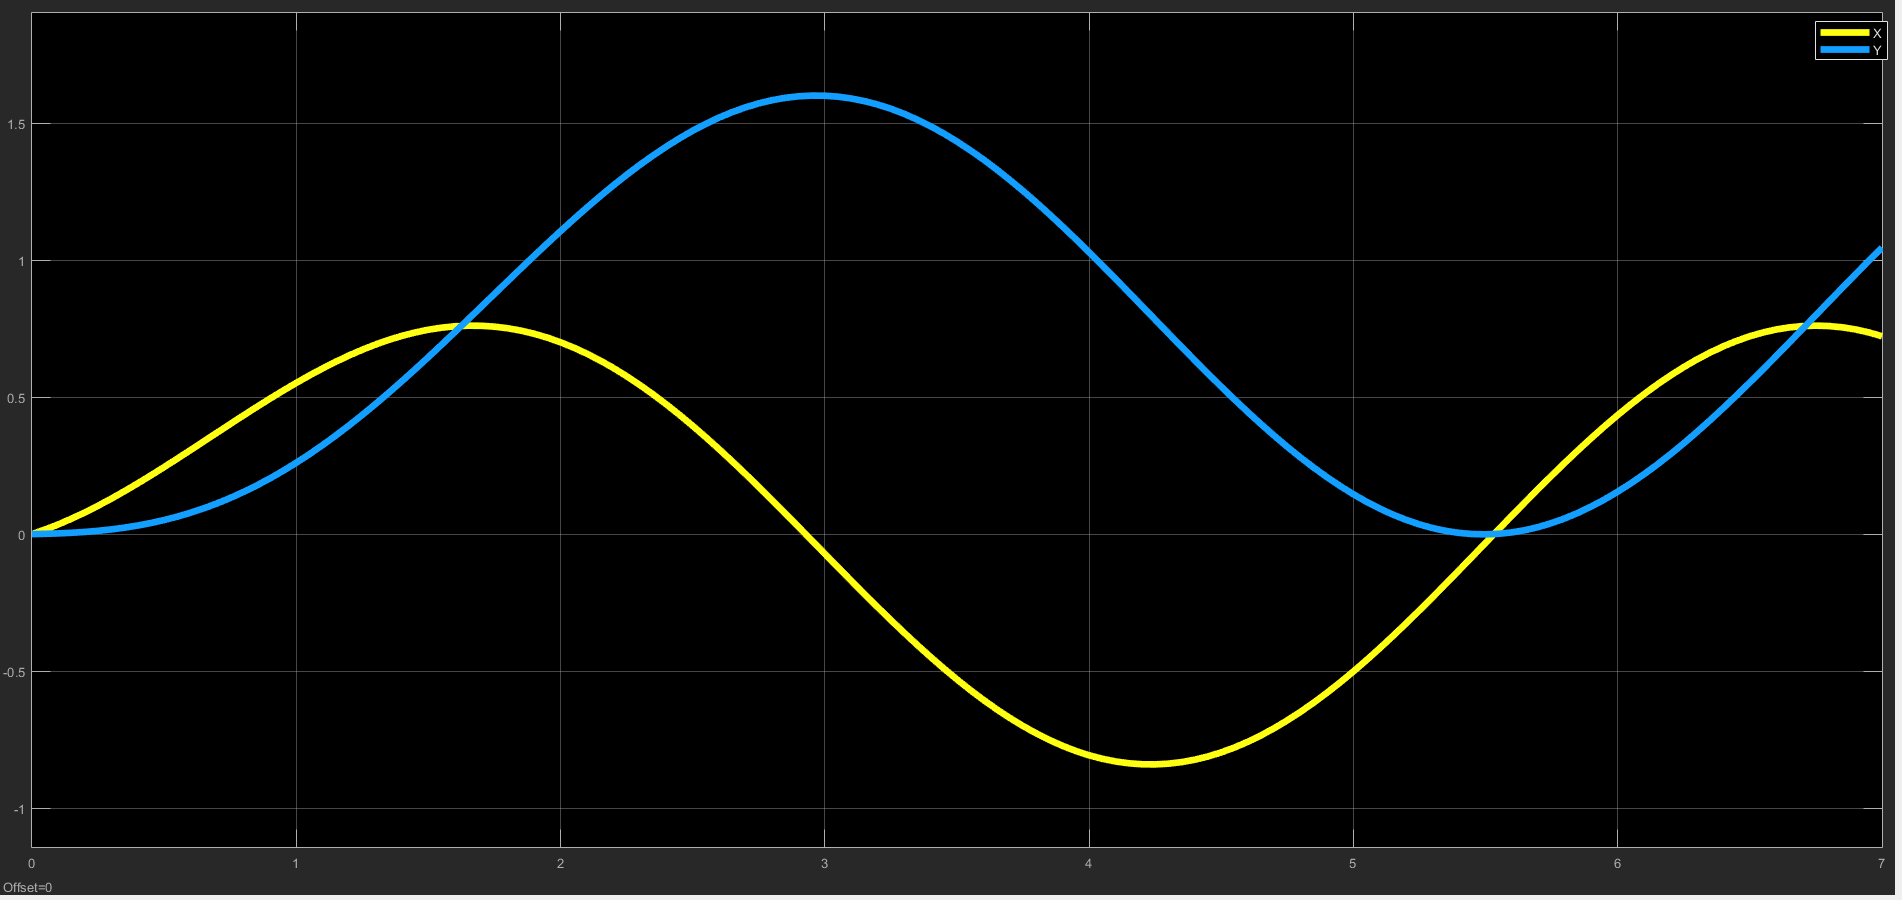
\includegraphics[width=1.0\textwidth]{./img/xy101.png}
\caption {\label{fig:sim2 - pos}Linear speed v=1m/s, teta=0.1rad}
\end{figure}
With this figure \ref{fig:sim2 - pos} it is possible to observe that both the
position of x and y of the car change with time. With a constant angle of tilt,
the car will turn constantly in the same direction, eventually making a 360
degrees turn and as the car as small dimensions, it takes a very small time for
it to do so, which is what is observed is this simulation.
%%% Local Variables:
%%% mode: latex
%%% TeX-master: "../../../dissertation"
%%% End:

\subsubsection{Obstacle Avoidance Through Odometric Sensors}
Wireless communication between devices is always prospect to errors and obstructions, as such a way had to be devised so that the rover will function safely when communications fail whilst also avoiding a significant decline in the system's life expectancy.\\In order to achieve this, several odometric sensors will be placed on the rover, covering the \ang{360} radius, and whenever it judges an obstacle is too close (through the feedback of the sensors) it will not follow commands that would force it to get any closer to said obstacle.\\The implementation of an autonomous obstacle avoidance algorithm was considered, however implementing such an algorithm would, in the best scenario, remove control from the user and, in the worst scenario, enter into direct conflict with the latter. Therefore, since neither of the aforementioned scenarios was in the best interests of either the system or the user, it was opted to simply force the system to stop if a command would take it too close to an obstacle and to not allow it to move towards it any further.
\subsubsection{Obstacle Avoidance Simulations}
In order to plot the rover's path on a 2D diagram, the \textit{Mobile Robotics Simulation Toolbox}, made available by MATLAB, will be used. A series of waypoints  (these will simulate the user's commands) will be placed on a 2D map with borders, the latter of which will be used as obstacles. The waypoints shall direct the rover towards one of the borders in a turn and a straight line. Ideally the rover will stop before reaching the obstacle whilst also keeping enough space to turn away from it.\\
\\
The initial position of the rover shall be at coordinates (1,1) and an angle of 0 rads, as depicted in Fig.~\ref{fig:iniState}. 
From this standpoint, two simulations will be considered: a straight line that will require a $\frac{\pi}{2}$ rads turn upward (this turn serves to test the algorithm, to make sure it does not stop changes in direction whilst away from obstacles) and head straight towards one of the walls of the map;
and a second simulation, involving a turn towards a wall. In order either simulation to be a success the rover must stop before crashing against the wall with enough space to steer away from the obstacle.

\begin{figure}[!htbp]
\centering
       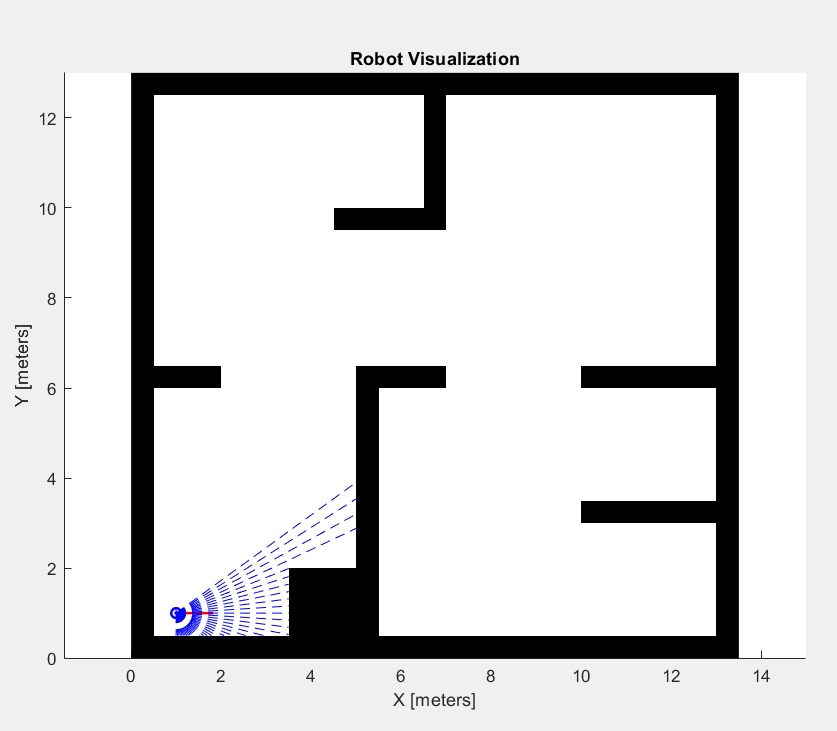
\includegraphics[page=1,width=0.55\textwidth]{img/startState.png} 
\caption{Initial State of simulation}
\label{fig:iniState}
\end{figure}

Firstly it must turn towards the wall, Fig~\ref{fig:sim1Turn}.
\begin{figure}[!htbp]
\centering
       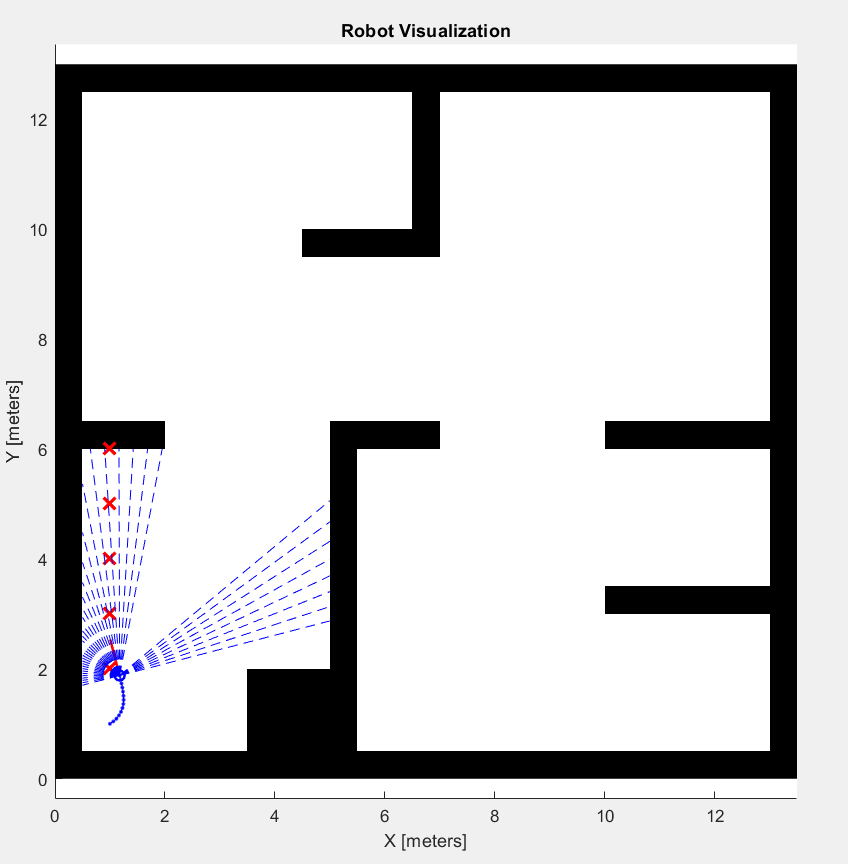
\includegraphics[page=1,width=0.55\textwidth]{img/line2.png} 
\caption{After Rover Turns Towards Wall}
\label{fig:sim1Turn}
\end{figure}

Afterwards it must head in a straight line and stop before the obstacle, Fig~\ref{fig:sim2Line}

\begin{figure}[!htbp]
\centering
       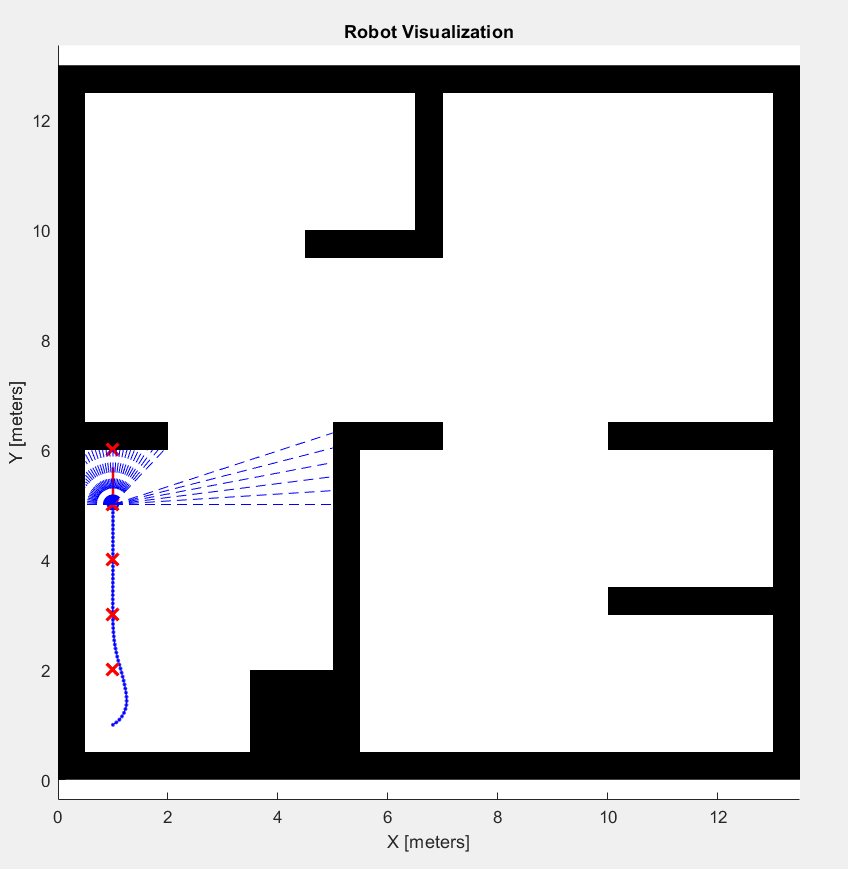
\includegraphics[page=1,width=0.55\textwidth]{img/line3.png} 
\caption{Rover Stopped Before Reaching Wall}
\label{fig:sim2Line}
\end{figure}

In the second simulation, which shall start, once again from the initial position depicted in Fig.~\ref{fig:iniState}, the rover must turn towards a path that avoids the right wall, Fig.~\ref{fig:sim2Line} and afterwards turn again and stop before reaching the wall with enough space to turn away from the latter, Fig.~\ref{fig:sim3Line}.

\begin{figure}[!htbp]
\centering
       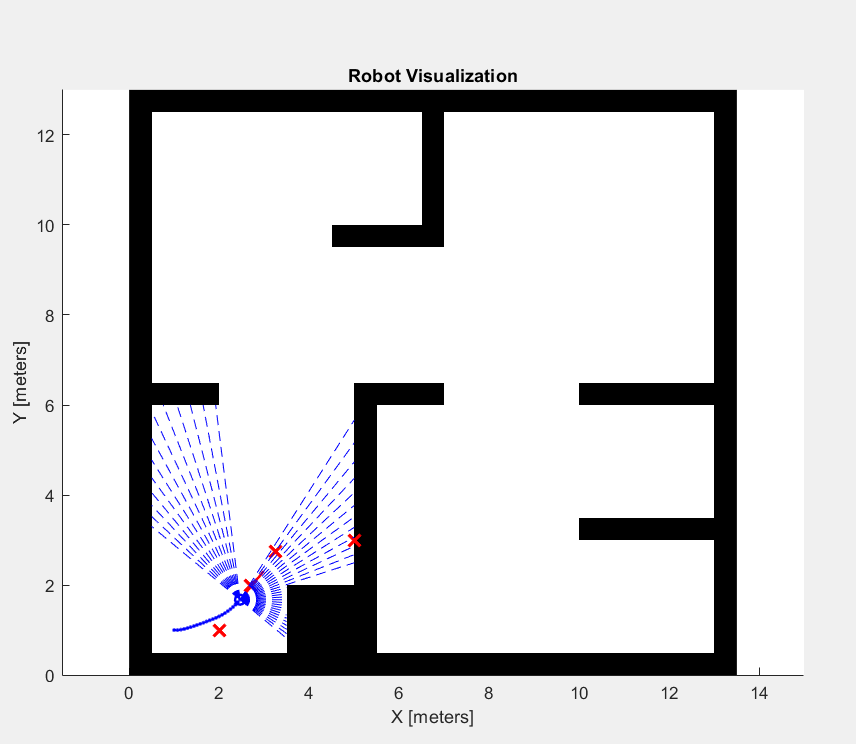
\includegraphics[page=1,width=0.6\textwidth]{img/turn2.png} 
\caption{Rover Starts the Turn}
\label{fig:sim2Line}
\end{figure}

\begin{figure}[!htbp]
\centering
       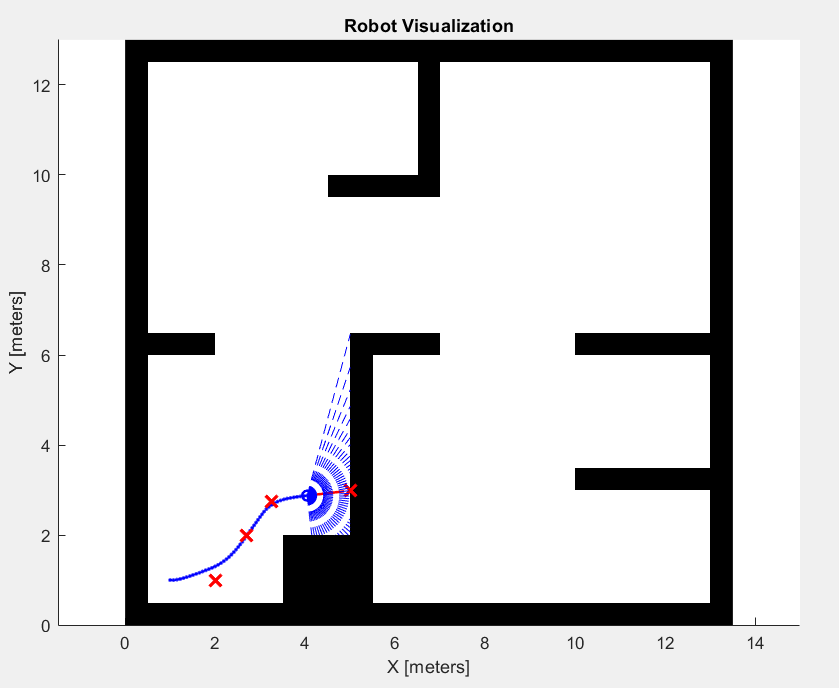
\includegraphics[page=1,width=0.6\textwidth]{img/turn3.png} 
\caption{Rover Turned and Stopped Before Reaching Wall}
\label{fig:sim3Line}
\end{figure}
\newpage

\subsubsection{Odometric Sensor} 
For the obstacle avoidance, several of \href{https://www.botnroll.com/pt/infravermelhos/158-sen-00242.html}{GP2Y0A21YK Infrared Sensors} (Fig~\ref{fig:sensor}) will be placed on the rover, since it has an allowable field angle of up to \ang{40}, this would mean at least 9 sensors would be required to cover \ang{360}, this is assuming that they are placed in such a way that there is no overlap, however since any sort of "blind spot" will place the rover in jeopardy, some overlap is desired. Considering the rover's dimensions, it is unlikely that 9 sensors can be placed upon it with enough overlap to completely cover the \ang{360}, therefore it is likely that a few more will have to placed to guarantee safety of the rover.

\begin{figure}[!htbp]
\centering
       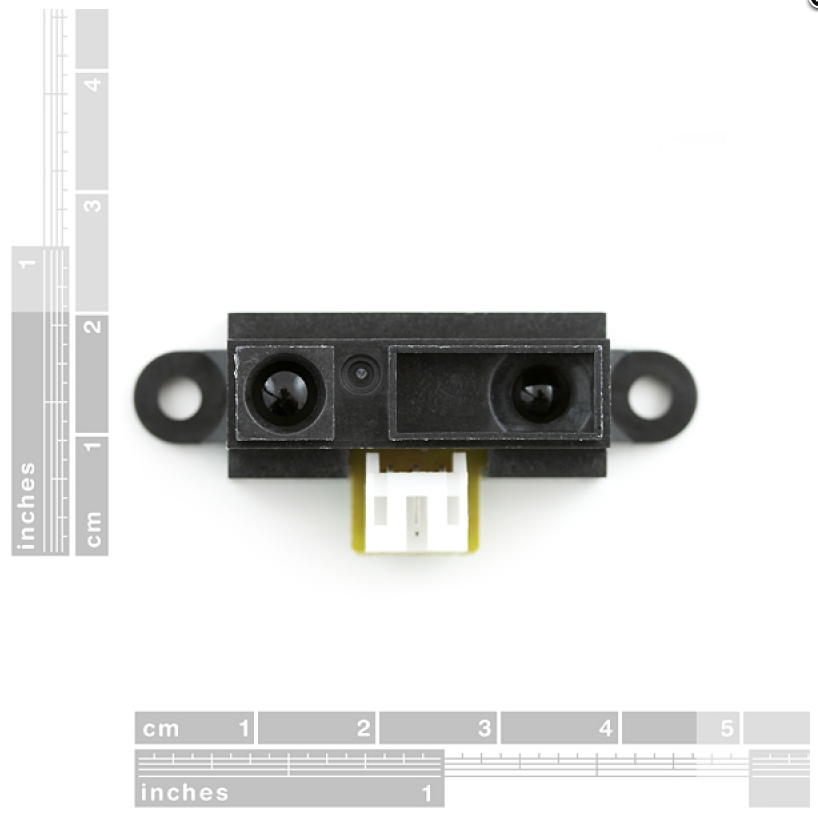
\includegraphics[page=1,width=0.35\textwidth]{img/sensor.png} 
\caption{Odometric Infrared Sensor GP2Y0A21YK}
\label{fig:sensor}
\end{figure}
%
\subsection{System design}%
\label{sec:navigation-system-design}
Tackling the objectives laid out in \cref{sec:navig-virt-subsyst-design} requires an organized and well thought-out plan of work because there are a lot of smaller systems at play that need to work cohesively and synchronously. 




%///////////////////////// # Separation into packages //////////////////////////

The best way to achieve a good plan is by first separating the problem into packages, and in each package have subpackages, each with a collection of modules dedicated to serve a collective purpose in the data treatment and organization chain. 

The system is divided into such packages as follows:

\begin{figure}[H]
	\centering
	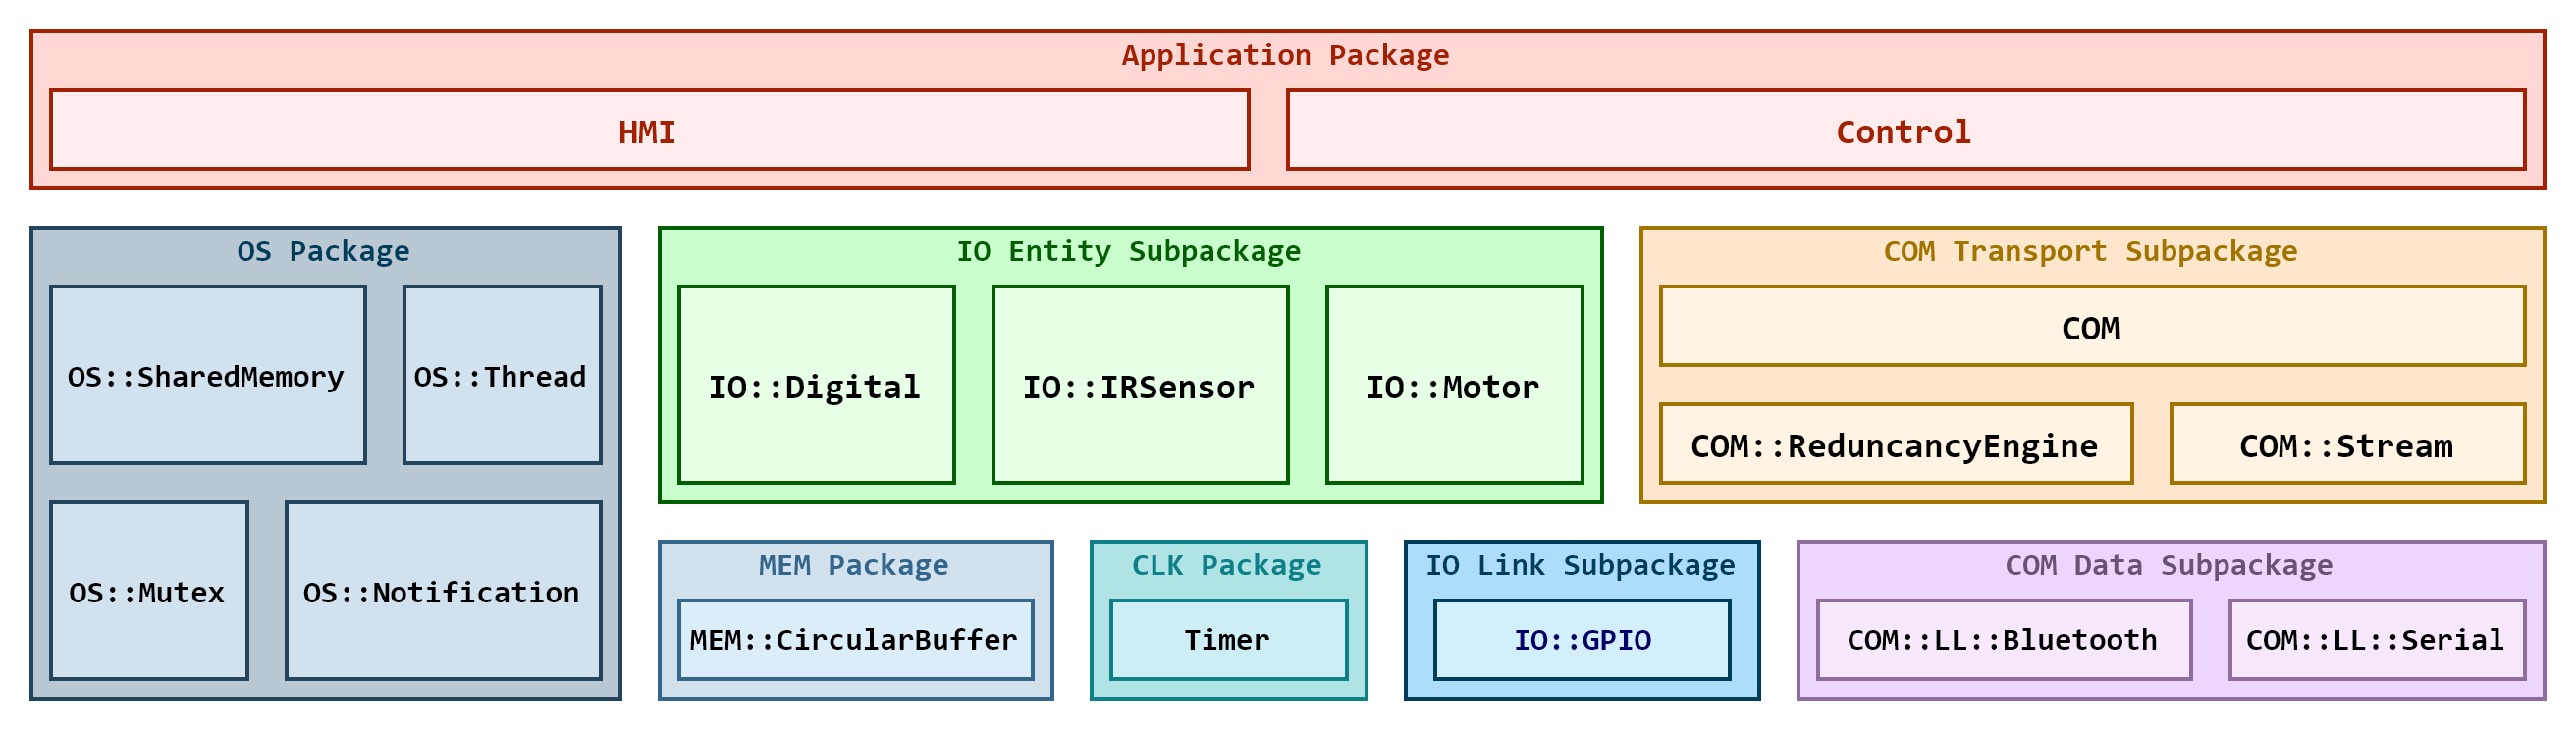
\includegraphics[width=1.0\textwidth]{./img/full-stack-overview.png}
	\caption {Full Stack Overview}
	\label{fig:full-stack-overview}
	\end{figure}
	


%////////////////////////// # Separation into layers ///////////////////////////

Each subpackage also belongs to a certain layer of software, characterized not by the resources it is associated to but by how close the modules within it are to the hardware. Futhermore, the packages should be distributed between layers in such a way that one seldomly need to use another that doesn't belong to the same layer or the layer directly below. 


These layers are, from the bottom to the top:
\begin{itemize}
	\item The High-level Hardware Abstraction Layer, which consists of the \textbf{OS} (partly), \textbf{MEM}, \textbf{CLK}, \textbf{IO Link} and \textbf{COM Data} packages/subpackages. Modules within this layer are responsible for the lower-level interaction with the system's resources so they are made to be thread-safe. Their implementation is platform-dependent and their interface is platform-agnostic. The main goal for this layer of software is to standardize the hardware, making for clean, maintainable and easily portable code. 
	\item The High-level Software Abstraction Layer, consisting of the \textbf{OS} (partly), \textbf{IO Entity} and \textbf{COM Transport} packages. The modules within these packages should serve as an interface with the lower level layer, creating a more intuitive interaction process and mechanisms for processing information asynchronously. This way, when other modules make use of those interfaces, the information is already parsed and ready to be retrieved.\\
	Modules in the layers above ara also highly dependent on both abstraction layers to carry out their tasks in time so the ones in this layer should provide robust mechanisms for exception-handling and timing. 
	\item The Main Application Layer, comprised only of the \textbf{APP} package, where the core functionality lies. As stated earlier, modules in this layer are protected from having to access to most lower-level layers but can use those modules and must use when no other abstraction is provided.
\end{itemize}


%//////////////////////////////// Static model /////////////////////////////////
\subsubsection{Static Model: Package diagram}

\begin{figure}[H]
	\centering
	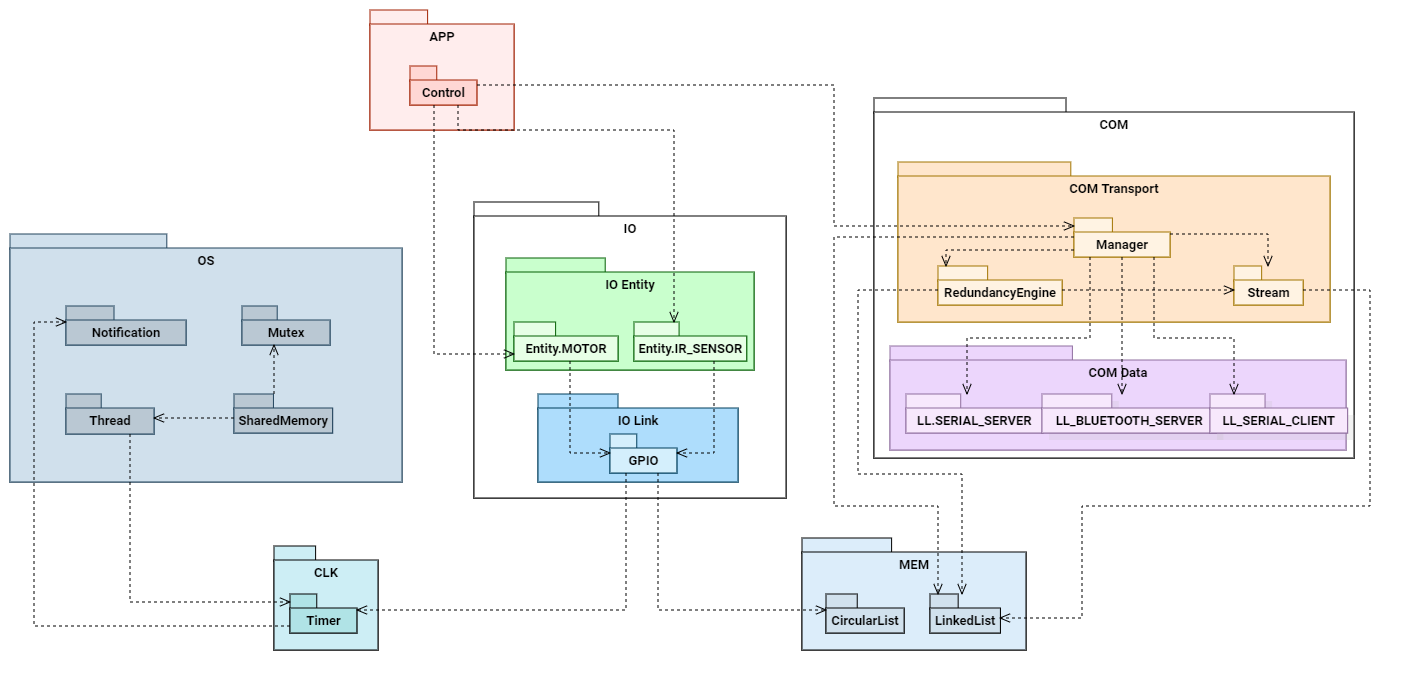
\includegraphics[width=0.8\textwidth]{./img/navig-package-diagram.png}
	\caption {Navigation subsystem package diagram}
	\label{fig:navig-package-diagram}
	\end{figure}



\subsubsection{Static Model: Class diagram}


\begin{figure}[H]
	\centering
	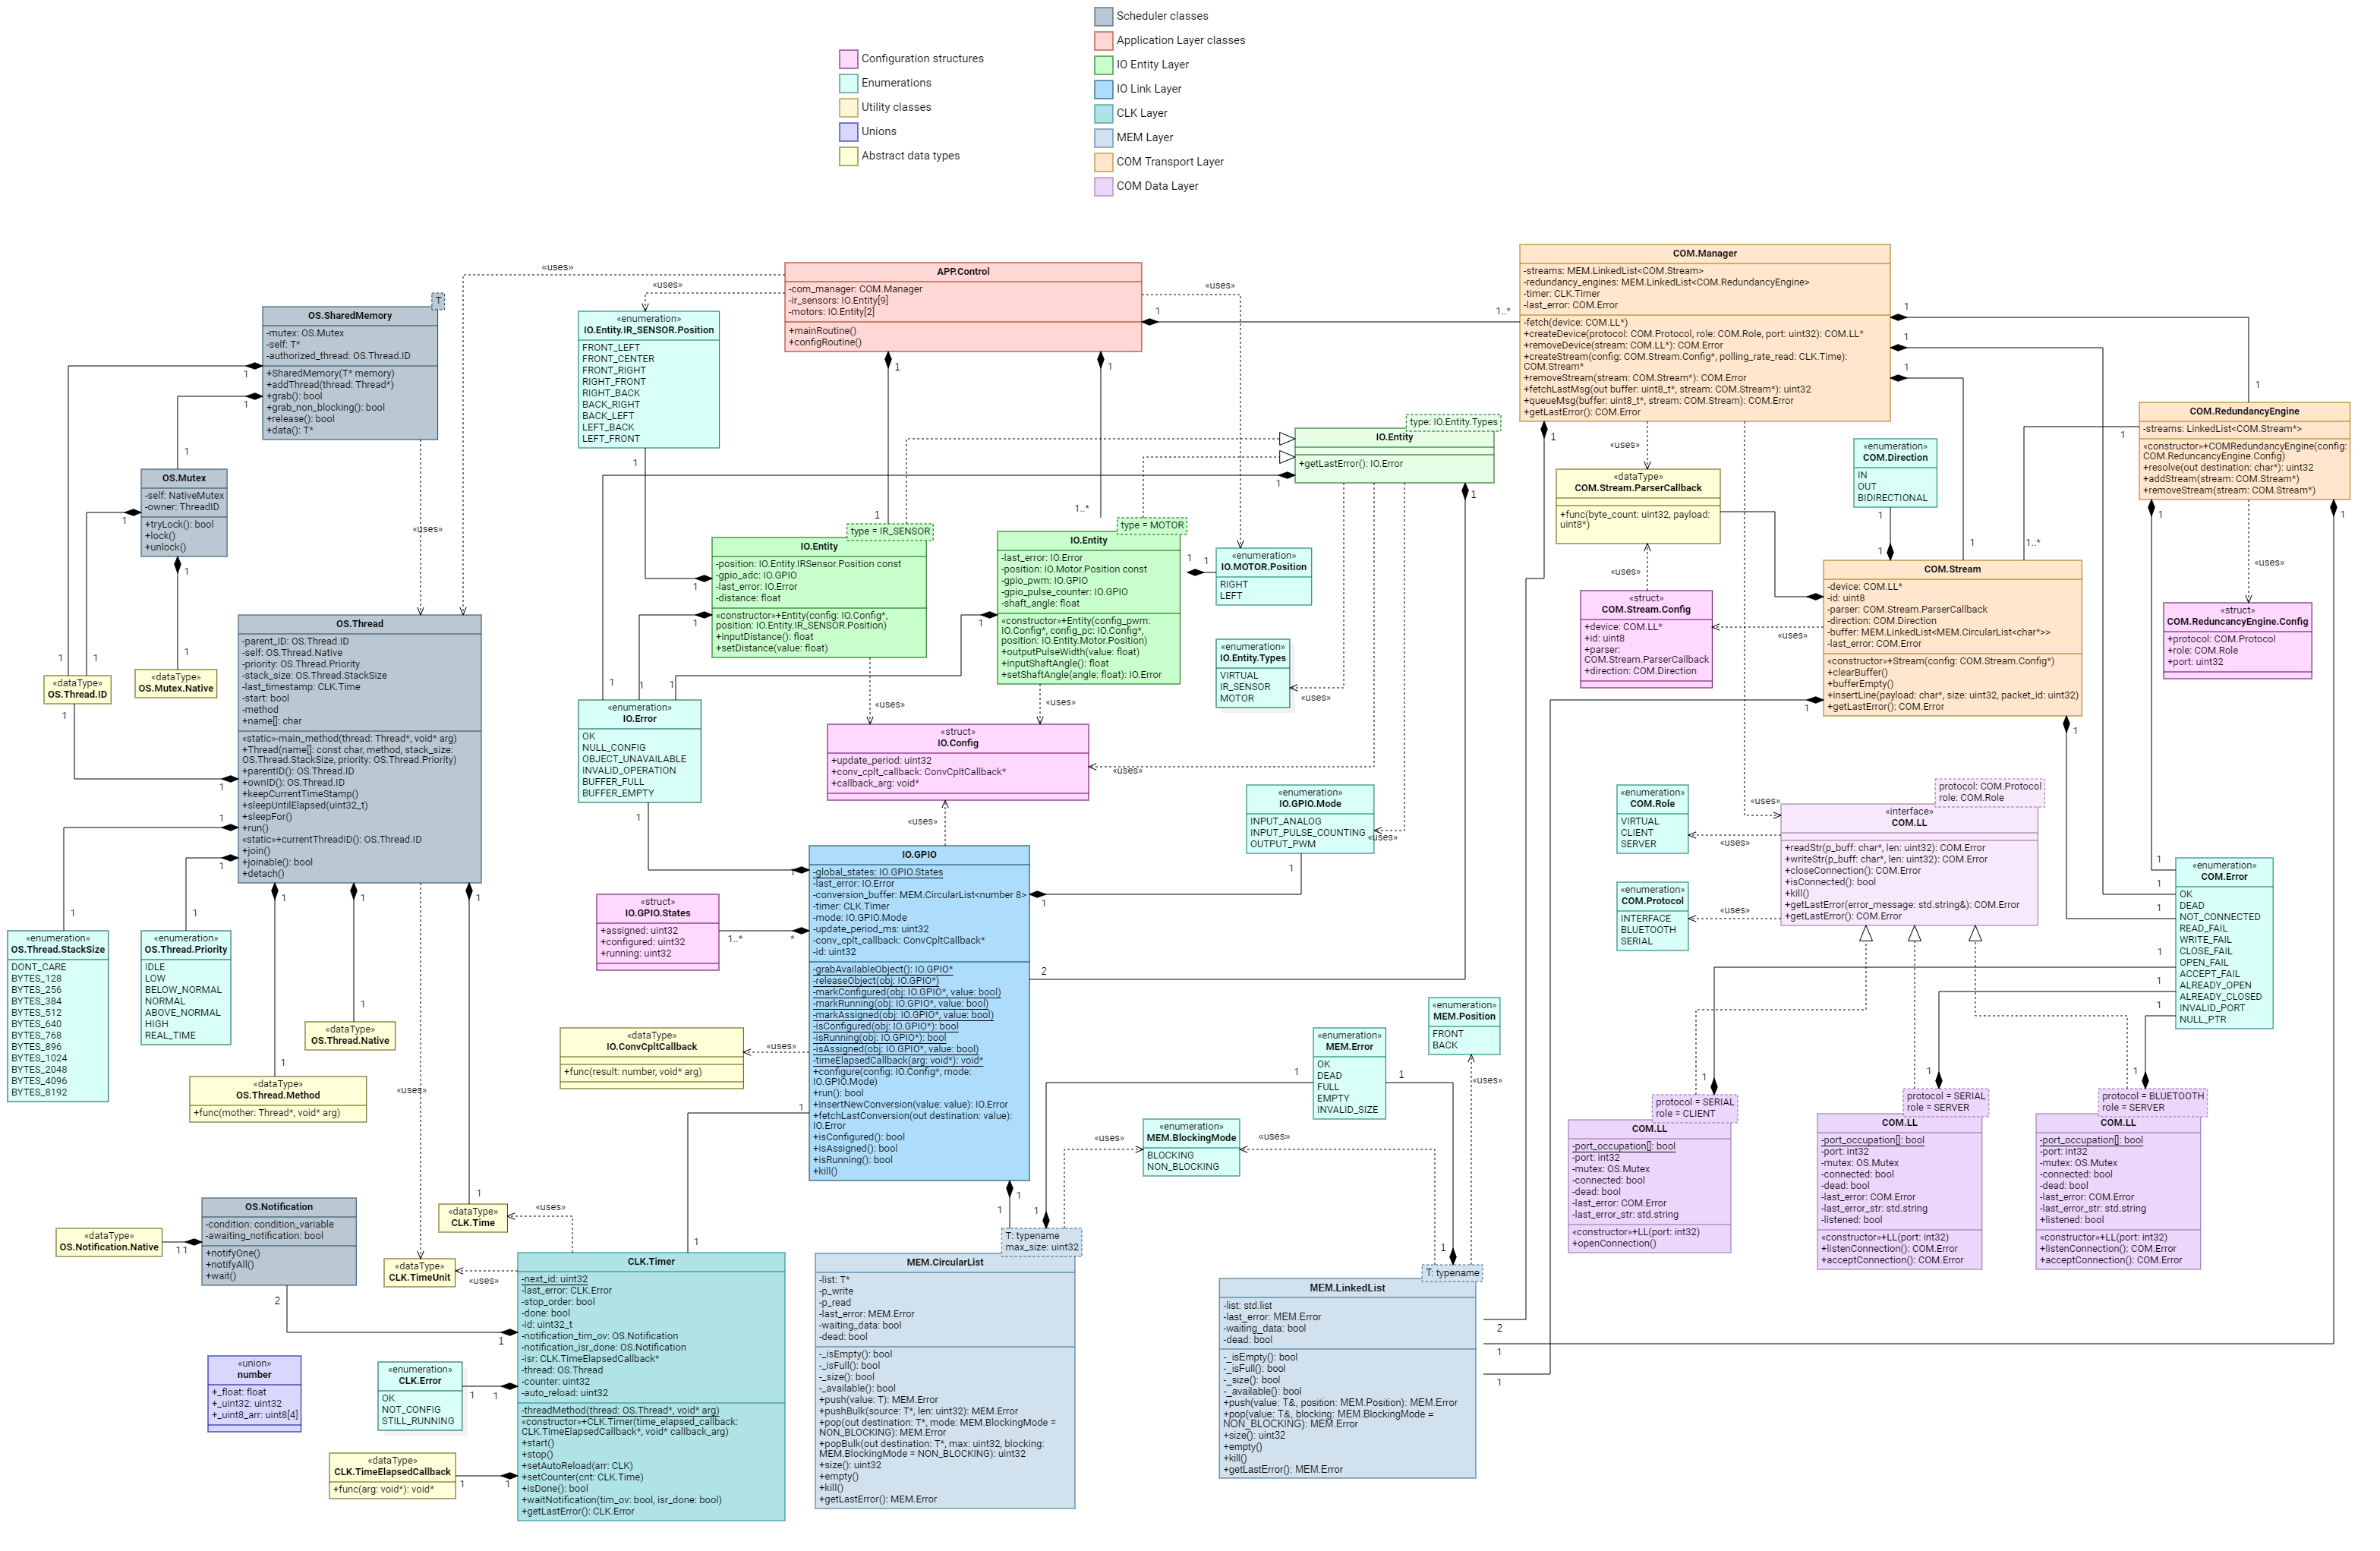
\includegraphics[width=\textwidth]{./img/navig-class-diagram.png}
	\caption {Navigation subsystem class diagram (augmented in Appendix \ref{fig:navig-class-diagram-augmented})}
	\label{fig:navig-class-diagram}
	\end{figure}



%//////////////////////////////// # IO Package /////////////////////////////////
\subsubsection{IO: Input/Output Package}
\label{sec:io-package}
The \textbf{IO} package is comprised of the \textbf{IO Entity} and \textbf{IO Link} subpackages. The modules within these subpackages are the parts of the hardware abstraction layers responsible for standardizing the General Purpose Input/Output resources of the machine.

The \textbf{IO Link} subpackage is the interface provides the most generic yet complete package for interacting with the machine. Its only module \textbf{IO::GPIO} provides such functionality as automatic resource assignment upon creation, automatic buffering of read and output values and the option of executing a specific piece of code when a conversion is completed for better effort distribution between layers.

\begin{figure}[H]
	\centering
	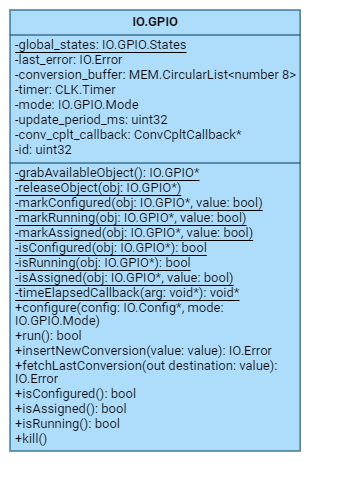
\includegraphics[width=0.38\textwidth]{./img/navig-class-gpio.png}
	\caption {IO::GPIO interface and members}
	\label{fig:navig-class-gpio}
	\end{figure}


The \textbf{IO::Entity} module from the \textbf{IO Entity} subpackage serves for specialization of functionality present in \textbf{IO Link} to serve a certain purpose attached to a physical meaning. This means it also extends the aforementioned callback mechanisms from \textbf{IO::GPIO} for automatic calculation of real-world values based on the measurements taken or otherwise that can be adapted and tailored further to serve the purpose of the specific application. Both provide a modest interface for storing important values calculated in the context of a \texttt{IO::ConversionCpltCallback} and a way to retrieve them.\\

Its \texttt{MOTOR} specialization uses an instance of \textbf{IO::GPIO} as an \texttt{INPUT\_PULSE\_COUNTING} to be able to count the number of pulses from the motor's encoder and output and one as an \texttt{OUTPUT\_PWM} to be able to output a pulse width modulated signal with a duty-cycle $D$ such that 
$$
V_{out average} = \frac{D\times V_{max}}{100}
$$

The \texttt{IR\_SENSOR} specialization uses an instance of \textbf{IO::GPIO} as an \texttt{INPUT\_ANALOG} for application in IR sensing applications. It provides a way to change the last calculated distance specifically for use in the corresponding callback function and an interface for retrieving that same value.

\begin{figure}[H]
	\centering
	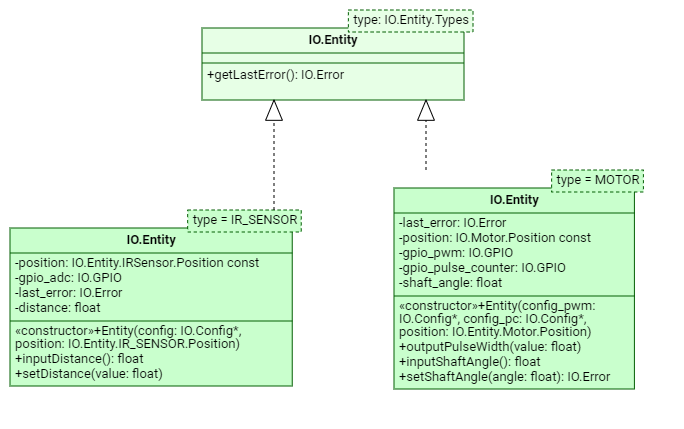
\includegraphics[width=0.65\textwidth]{./img/navig-class-entity.png}
	\caption {IO::Entity interface and specializations' methods and members}
	\label{fig:navig-class-entity}
	\end{figure}



\begin{figure}[H]
	\centering
	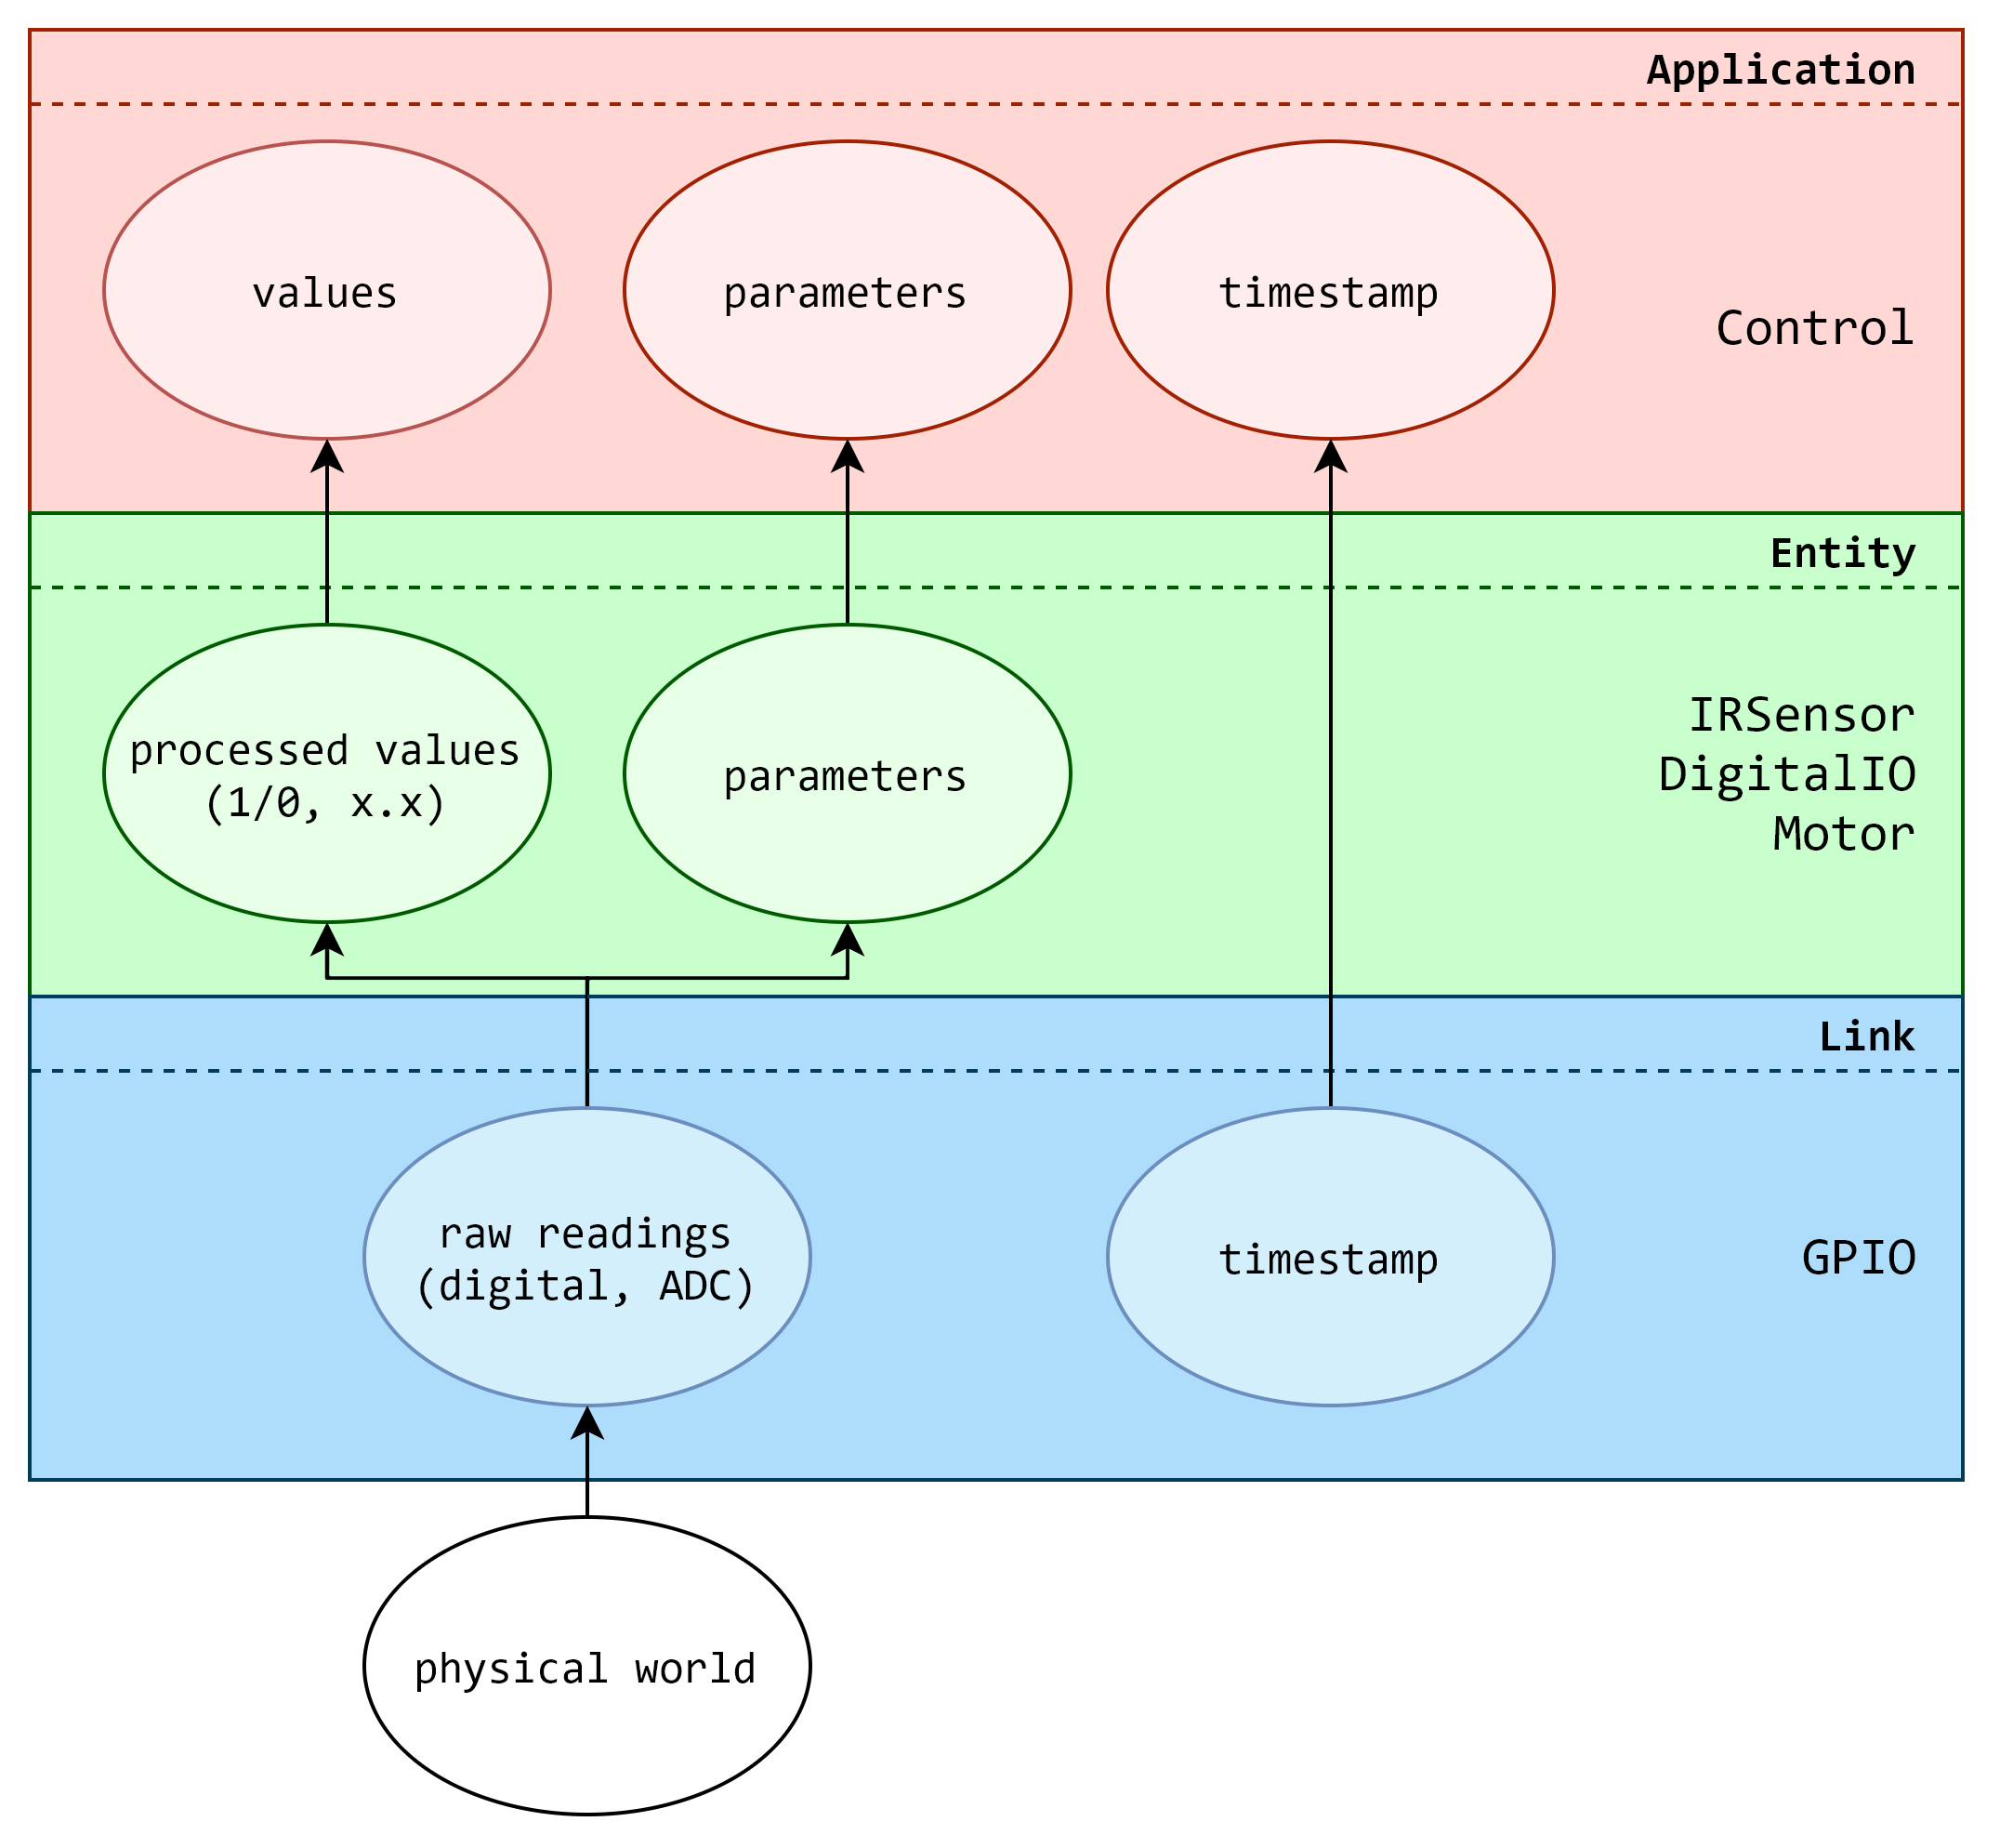
\includegraphics[width=0.5\textwidth]{./img/module-stack-io.png}
	\caption {IO subpackage interaction and information propagation diagram}
	\label{fig:navig-module-stack-io}
	\end{figure}

 

%//////////////////////////////// # COM Package ////////////////////////////////
\subsubsection{COM: Communications Package}

The COM package is the sum of the COM Data and COM Transport subpackages. These  modules are responsible for standardizing the access to the inter-device communication resources of each machine. 


The \textbf{COM Data} subpackage is aimed at providing a platform-agnostic interface for communicating over a serial or Bluetooth connection, while also providing specific functionality for different protocols/roles.
The \textbf{COM Transport} subpackage provides tools for managing multiple simultaneous, redundant, multiprotocol and multi-stream connections as well as automatically parsing of data for usage in time-constrained scenarios.

\begin{figure}[H]
	\centering
	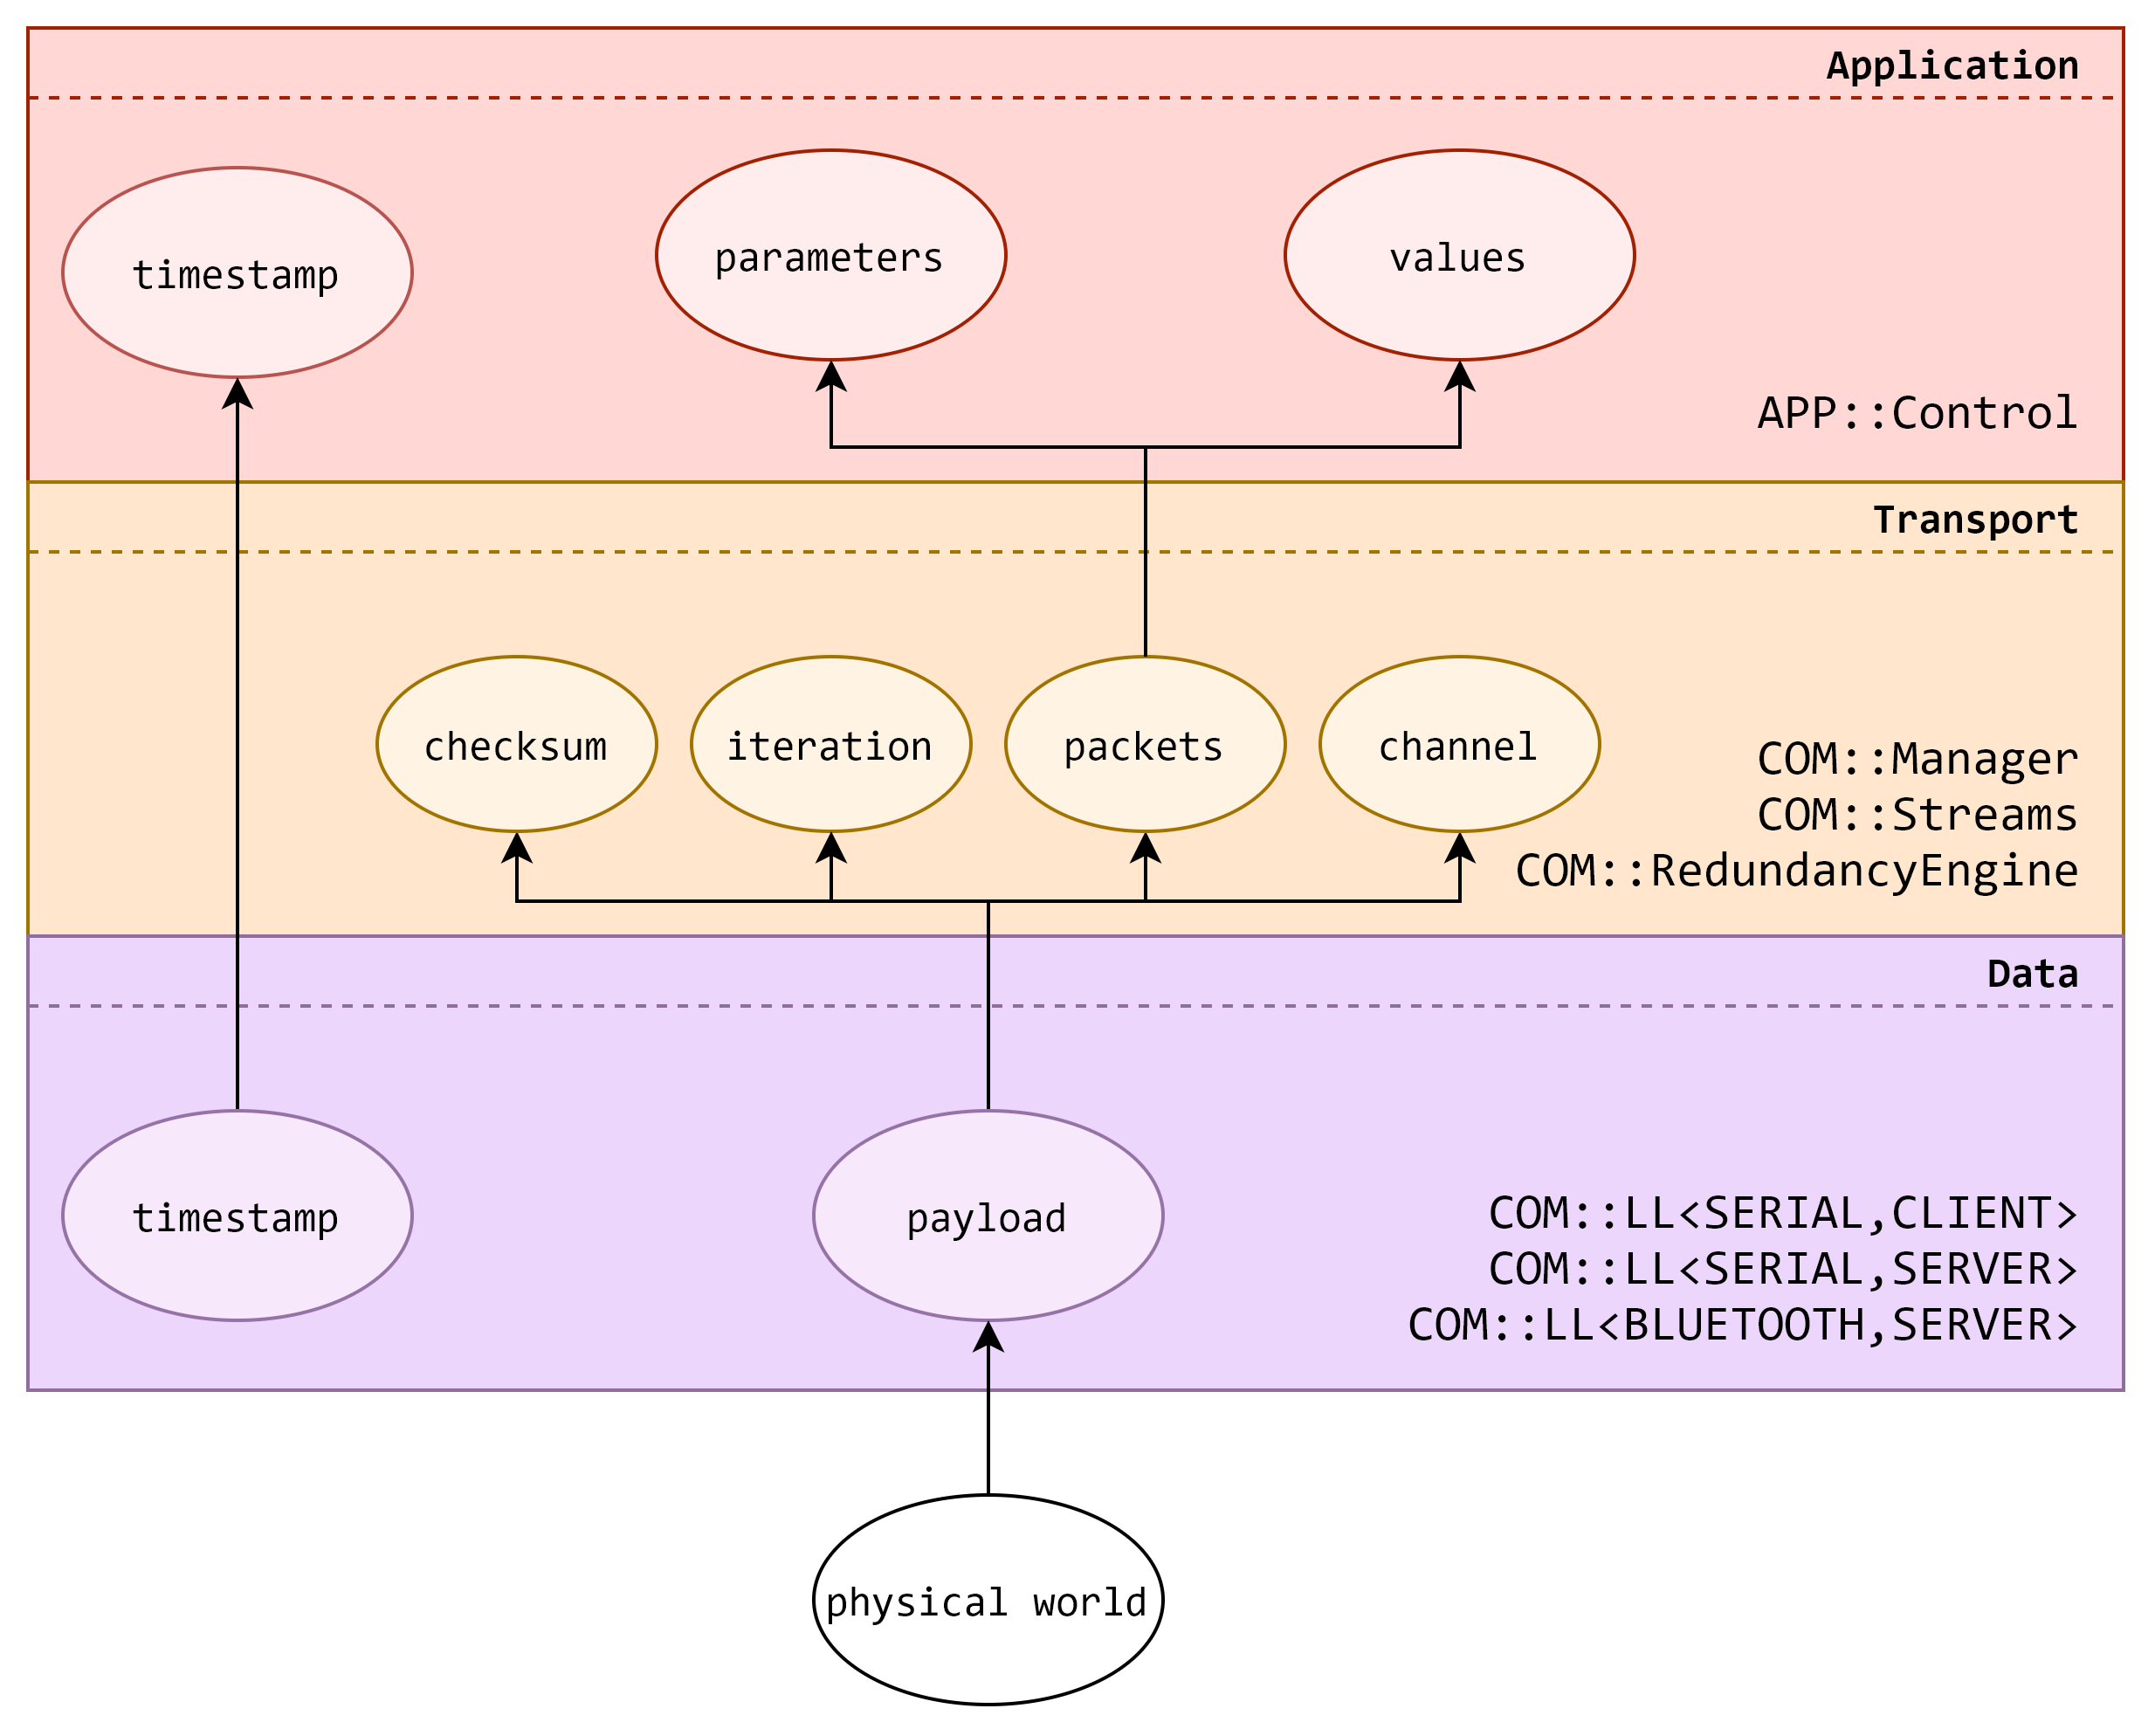
\includegraphics[width=0.5\textwidth]{./img/module-stack-com.png}
	\caption {COM subpackage interaction and information propagation diagram}
	\label{fig:navig-module-stack-com}
	\end{figure}



The \textbf{COM::LL} module makes up the lower layer of the COM package. It should then have very well defined and error-tolerant behaviour and a somewhat familiar interface. With that in mind, it had an error-reporting system that would give feedback over a variery of errors such as invalid ports or non existing connections. It has been envisioned to be capable of connecting devices through serial and bluetooth protocols using a typical client and server socket model.

\begin{figure}[H]
	\centering
	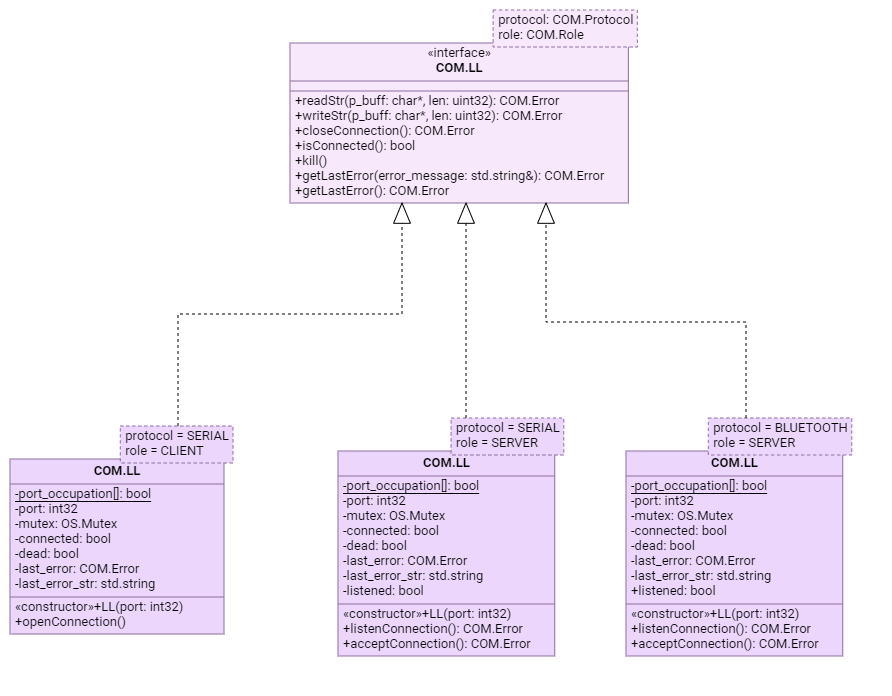
\includegraphics[width=0.8\textwidth]{./img/navig-class-ll.png}
	\caption {COM::LL interface and specializations' methods and members}
	\label{fig:navig-class-ll}
	\end{figure}


The \textbf{COM::Stream} module allows the partitioning of communications effected through the same medium into streams, resulting in well established boundaries which simplify any information processing required. It allows the formatting of any message into a recognizable packet complete with all the required metadata, for packet and stream identifications and simple error detection. It also permits the establishment of callbacks for effort distributing in parsing the information.

\begin{figure}[H]
	\centering
	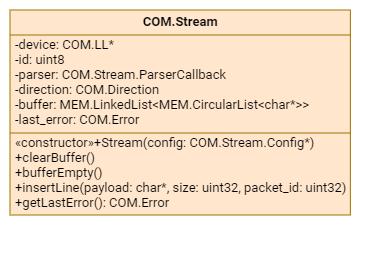
\includegraphics[width=0.4\textwidth]{./img/navig-class-stream.png}
	\caption {COM::Stream interface and members}
	\label{fig:navig-class-stream}
	\end{figure}


The \textbf{COM::RedundancyEngine} module allows several related streams "connect" and "disconnect" to and from it and compares the information between them resolving conflicts and missing information. The latter of which can be accessed through a call \texttt{resolve()}.

\begin{figure}[H]
	\centering
	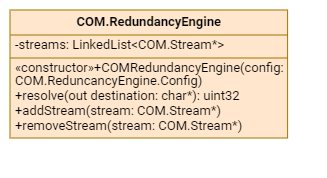
\includegraphics[width=0.35\textwidth]{./img/navig-class-redundancy-engine.png}
	\caption {COM::RedundancyEngine interface and members}
	\label{fig:navig-class-redundancy-engine}
	\end{figure}


The \textbf{COM::Manager} module is a higher level when compared to the others, it connects the tools of the other modules to create an interface that allows quick and intuitive communication setup and automatization of processes such as redundancy management.
\begin{figure}[H]
	\centering
	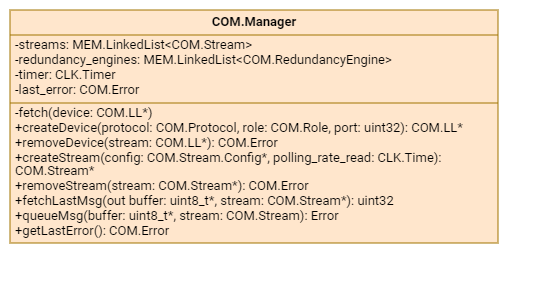
\includegraphics[width=0.5\textwidth]{./img/navig-class-manager.png}
	\caption {COM::Manager interface and members}
	\label{fig:navig-class-manager}
	\end{figure}



%//////////////////////////////// # OS Package /////////////////////////////////
\subsubsection{OS: Scheduler Package}
\label{sec:osPack}
The modules in the \textbf{OS} package mainly serve the purposes of thread creation and management management, inter-thread synchronization and thread-safe access to memory. Therefore, they all revolve around threaded execution although each fills in the need for a special bit of functionality.

The \textbf{OS::Thread} module provides a platform-agnostic interface for creating an object that will use native types and interfaces that allow each object to behave like a separate execution thread. The provided controls for it include execution and sleep mechanisms as well as options for waiting for the end of their execution and detaching threads from the parent thread. Scheduling can be managed with the options concerning thread priority and for the possibility of creating static threads it also provides the chance of delimiting the stack size. 

\begin{figure}[H]
	\centering
	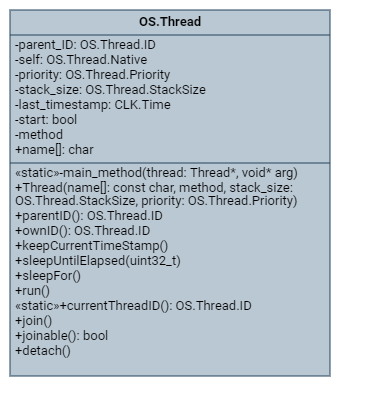
\includegraphics[width=0.4\textwidth]{./img/navig-class-thread.png}
	\caption {OS::Thread interface and members}
	\label{fig:navig-class-thread}
	\end{figure}


The \textbf{OS::Mutex} module provides a way for controlling access to shared resources that are not defined as thread-safe, which is any object that the user might create that is not of any of the modules in the High-level Hardware Abstraction Layer. It can be locked (\texttt{lock()}) in one thread in order to block access to a specific excerpt of code and it can only be locked again by the same thread or any other after it is unlocked (\texttt{unlock()}) by whatever thread locked it. It is thus non-recursive, which means that any thread, including the thread that locked in blocked in the call to \texttt{lock()} it until it is unlocked.

\begin{figure}[H]
	\centering
	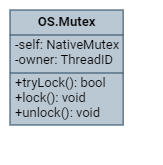
\includegraphics[width=0.15\textwidth]{./img/navig-class-mutex.png}
	\caption {OS::Mutex interface and members}
	\label{fig:navig-class-mutex}
	\end{figure}


The \textbf{OS::SharedMemory} module, one the other hand, provides a platform for sharing resources between specific threads. It may be considered an expansion upon \textbf{OS::Mutex} that is specifically tailored to be used in memory protection and can reduce the roster of threads that get access to a certain memory area. 


\begin{figure}[H]
	\centering
	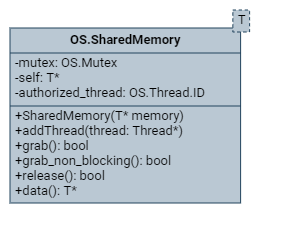
\includegraphics[width=0.25\textwidth]{./img/navig-class-sharedmemory.png}
	\caption {OS::SharedMemory interface and members}
	\label{fig:navig-class-sharedmemory}
	\end{figure}


\textbf{OS::Notification} is a small module that provides the inter-thread synchronization method known as a signal or a notification. A call to \texttt{wait()} from one thread will make it halt until a call for \texttt{notifyOne()} that targets it is given from another thread. A call to \texttt{notifyAll()} will notify all threads. 


\begin{figure}[H]
	\centering
	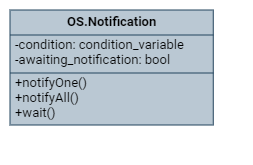
\includegraphics[width=0.28\textwidth]{./img/navig-class-notification.png}
	\caption {OS::Notification interface and members}
	\label{fig:navig-class-notification}
	\end{figure}


\subsubsection{MEM: Memory Structures Package}

The \textbf{MEM} package includes modules that offer typical containers such as linked lists and circular lists that are tightly contained and thread-safe. These are very practical ways of implementing those types of structures in heavily threaded applications as they provide easy-to-use interfaces, low-complexity operations and guarantee safe access to the resources when shared by multiple threads. 
\newline
Both \textbf{MEM::CircularList} and \textbf{MEM::LinkedList} provide interfaces for inserting and removing objects, retrieving basic information about their state, such as their size and a means to empty the list in an efficient fashion. They both also implement the universal error reporting interface with a specific type for such errors, \textbf{MEM::Error}. When making specific operations the user can also choose how the container should react when another thread of execution is accessing the structure: in \textbf{MEM::BlockingMode BLOCKING} mode, the list will wait until the resources are freed and in \textbf{NON\_BLOCKING} mode, in the same situation it will return with an error code.
\newline
The \textbf{MEM::CircularList} provides a medium for creating a fixed-size First-In-First-Out (FIFO) container to which the user can push a single or multiple objects and retrieve them in a similar fashion. 

\begin{figure}[H]
	\centering
	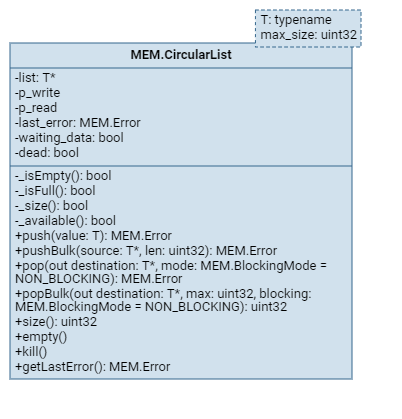
\includegraphics[width=0.4\textwidth]{./img/navig-class-circularlist.png}
	\caption {MEM::CircularList interface and members}
	\label{fig:navig-class-circularlist}
	\end{figure}

The \textbf{MEM::LinkedList} prioritizes quick insertion at the front or the back of any list and removal of specific objects from anywhere in the list with the same complexity. It it optimized exclusively for operations with single objects.

\begin{figure}[H]
	\centering
	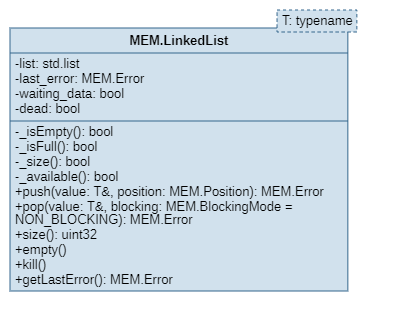
\includegraphics[width=0.4\textwidth]{./img/navig-class-linkedlist.png}
	\caption {MEM::LinkedList interface and members}
	\label{fig:navig-class-linkedlist}
	\end{figure}


The modules within this package are mainly used by the \textbf{IO} and \textbf{COM} class modules for buffering information and storing objects in lists where insertions and removals need to be fast but they can also be used by higher-level classes due to their \textbf{versatile interfaces} and \textbf{general-purpose} nature.


%//////////////////////////////// # CLK Package ////////////////////////////////

\subsubsection{CLK: Timing Package}

The \textbf{CLK} package is comprised by only the \textbf{Timer} module and convenient type definitions. It provides a means for setting up repeated timed delays and executing a specific routine automatically when each delay ends. It also provides an interface for waiting for the end of the timed delay and/or the execution of the specified routine and autonomously notifies all waiting objects of these events.
It is mainly used by the \textbf{IO::GPIO} class for timing conversions but it can as easily be used by higher-level classes due to its \textbf{versatile interface} and \textbf{general-purpose} nature.

\begin{figure}[H]
	\centering
	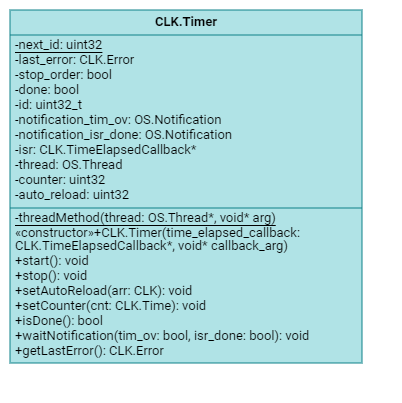
\includegraphics[width=0.43\textwidth]{./img/navig-class-timer.png}
	\caption {CLK::Timer interface and members}
	\label{fig:navig-class-timer}
	\end{figure}



%//////////////////////////////// # APP Package ////////////////////////////////

\subsubsection{APP: Main Application Package}

The main application package is comprised by  


%
\section{Physical Environment Virtual Subsystem}%
\label{sec:phys-envir-virt-design}
%The Navigation subsystem hosts the core of the system functionality-wise, which is the control routine. This means that it should strive to not only make accurate readings and calculations but also be as efficient as possible in managing those processes in order to introduce very little delay and meet timing requirements. 

To meet these requirements as best as possible it should be capable of :

\begin{itemize}
    \item Gathering information from the physical domain at equally distant instants $kT_s$ and output an electrical representation of the command variable at equally distant instants $kT_o$;
    \item Acquiring commands from the Smartphone and Remote Vision Subsystems, identifying matches that will allow it to validate those commands and feeding them into the control rule in a useful format;
    \item Providing real-time feedback to the user about its status.
\end{itemize}


The first task should be idealizing the control system itself, understanding what inputs are needed to control the machine and then how it could be used to manipulate the wheels of the car. After that, the rest of system should be designed to fit the needs of the control rules and algorithms and use them to react as fast and consistently as possible within its own constraints and those of the other subsystems.
%
%\section{Remote Vision Virtual Subsystem}%
%\label{sec:remote-visi-subsyst-design}
\section{Remote Vision Virtual Subsystem}%
\label{sec:remote-visi-subsyst-design}
The design specification devised in
Section~\ref{sec:remote-visi-subsyst-design} can now be implemented to the
target platform to fulfill the remote vision and telemetry functionalities
required. In this section the relevant implementation details are
addressed on the hardware and software domains.
%
\subsection{Hardware}%
\label{sec:hardware-rvvs-implem}
In the design stage, and in the first iterations of the
implementation, it is perfectly reasonable to adopt general domain environments,
such as virtual machines. Nonetheless, one must keep in mind that, ultimately,
the devised software will be running on hardware nodes. Thus, an important implementation step is the selection of the target
platform, taking into considerion several design criteria, such as, throughput,
memory footprint, storage, response time, connectivity, etc.

An example of a viable platform is the Raspberry Pi Zero W (Fig.~\ref{fig:pi-zero-w}), which is a low cost
board design (it retails for about 5 EUR) around the Broadcom system on-chip (SoC) BCM2835, which includes a
1 GHz single-core ARMv6 CPU, with a 64-bit architecture, allowing it to run
the full range of GNU/Linux distribution. Among other resources, it includes 512
MB RAM, VideoCore IV GPU, 40 GPIO pins, mini HDMI and micro-USB ports,
\gls{csi} connector, Micro SD Card Slot and on-board Bluetooth Low Energy (BLE)
4.1 and Wi-Fi based.

The Raspberry Pi Zero W provides the required communications
(Bluetooth and Wi-Fi) and camera interfaces, on a fully-fledged environment
capable of running 64-bit OS and at low cost, thus, making it
suitable for the implementation. Additionally, it packs in a small form-factor,
even with the inclusion of the camera, as illustrated in
Fig.~\ref{fig:pi-zero-w-cam}. The camera module has several models ranging from
5 to 12 megapixel resolution with high quality video capture (up to 1080p30) in
the 20--35 EUR pricepoint.
%
% Pi Zero W
\begin{figure}[!hbt]
\centering
    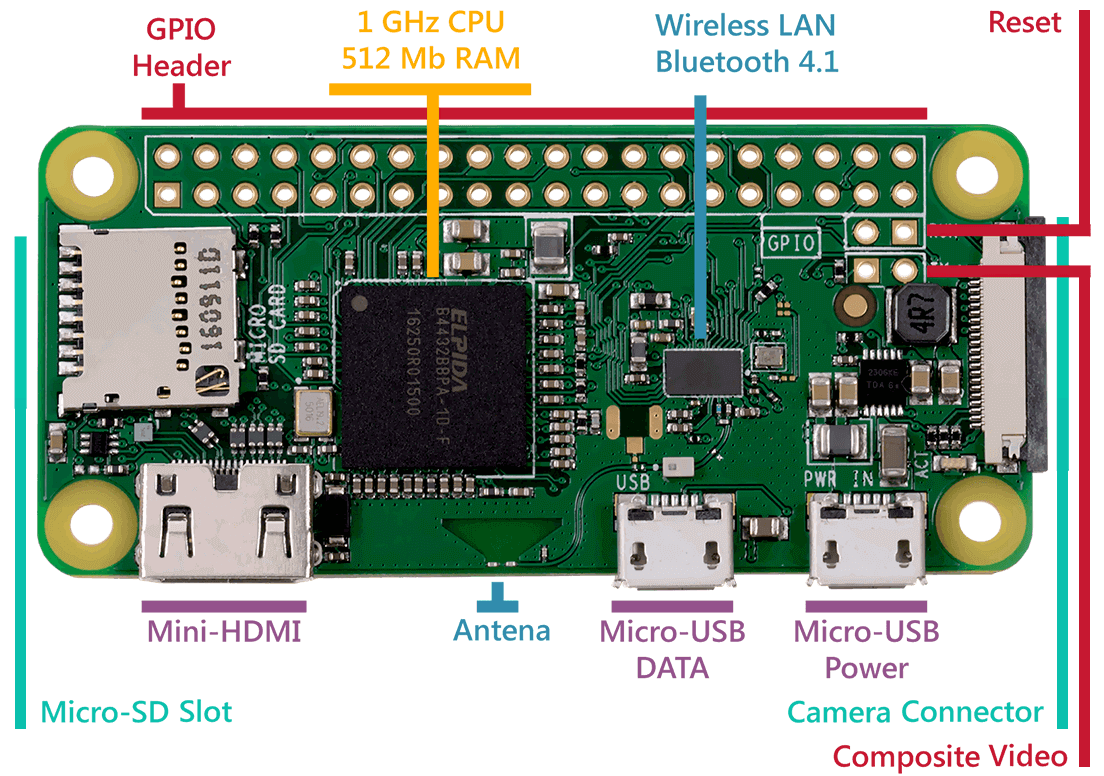
\includegraphics[width=0.6\textwidth]{./img/pi-zero-w.png}
  \caption{Raspberry Pi Zero Wireless overview}%
\label{fig:pi-zero-w}
\end{figure}
% Pi Zero W Camera
\begin{figure}[!hbt]
\centering
    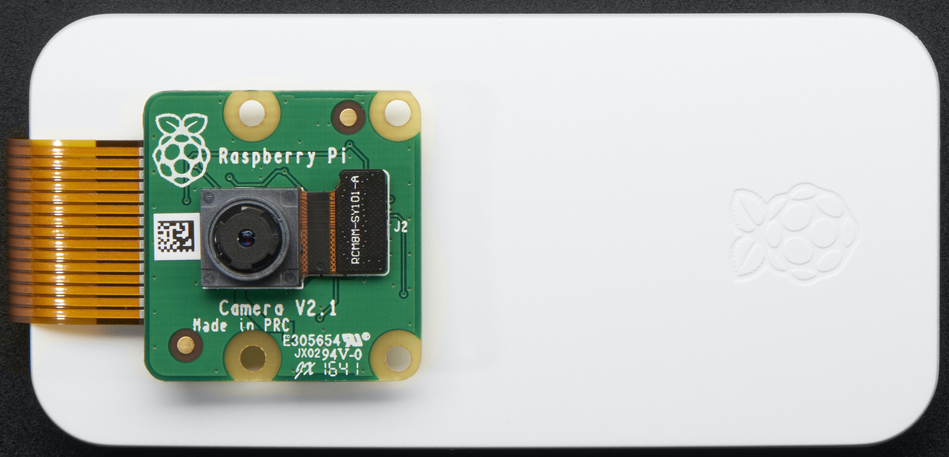
\includegraphics[width=0.6\textwidth]{./img/pi-zero-w-cam.jpg}
  \caption{Raspberry Pi Zero Wireless overview}%
\label{fig:pi-zero-w-cam}
\end{figure}
%
%
\subsection{Software}%
\label{sec:software-rvvs-implem}
The software part is mainly comprised of two main components: the software
environment support and the actual software running on top of that. The software
environment provides the low-level layer(s) that interfaces the hardware,
typically under some form of an \gls{os} and the associated development
toolchain required to target the platform.

In the present case, the selected platform --- Raspberry Pi --- supports
64-bit GNU/Linux based operating systems, which can be used to bootstrap the
implementation. Nonetheless, it is desirable to maintain the code footprint and
dependencies as low as possible, as required in the majority of the embedded
systems, thus, a custom tailored Linux OS can be used. Contemplating the build
tools required for the deployment of a tailored Linux OS, there are several
solutions, such as, Buildroot, Yocto and OpenWRT. The selected build tool was
Yocto, an open-source project project that provides templates, tools, and
methods to help you create custom Linux-based systems for embedded products
regardless of the hardware architecture~\cite{yocto2020}. Additionally, it is
required the cross-compilation toolchain that enables deployment to target from
host. Yet, in this initial implementation phase, the \gls{rvvs} susbsystem is
virtualized in a Linux \gls{vm}, thus, sparing this step for now. However, after
implementing and testing the application in the Linux \gls{vm}, this approach
should be relatively straightforward, enabling fast deployment to the real
hardware.

Hence, in the following sections, it is discussed the implementation of the
\gls{rvvs} stack designed in Section~\ref{sec:subsyst-decomposition-rvvs}.
%
\subsubsection{Image Acquisition}%
\label{sec:img-acq-rvvs-implem}
The usage of the Linux \gls{vm} has another inherent advantage, associated to
the UNIX philosophy in which it is based, that everything is a file (except for
the network part). As a matter of fact, every device attached to the Linux OS
can be easily and transparently accessed, e.g., via the \texttt{/dev}
directory. Additionally, as every device is a file, the file \gls{api} can be
used to manage the device, using the typical system calls \texttt{open/close}
and \texttt{read/write}.  

The typical call stack for image acquisition and streaming is comprised of:
low-level drivers that interface the hardware via the kernel (dependent on the
type of interface), dealing with frame capture (e.g., \gls{v4l}); and the
commonly named \emph{frame grabber}, which takes the raw frames and encodes it
into streams, for posterior multiplexing into their final container (e.g.,
\texttt{ffmpeg}).

The \gls{v4l2} is the second version of the \gls{api} and framework, which is an
integral part of the Linux kernel code, as opposed to many driver
implementations~\cite{v4l2-headers}. The \gls{v4l2} \gls{api} is mostly
implemented as set of \texttt{ioctl} (control device) system
calls~\cite{kerrisk2010linux} that enable easy manipulation of video devices.
\emph{The workflow for a typical \gls{v4l2} application is as follows}:
\begin{enumerate}
\item Open a descriptor to the device;
\item Retrieve and analyse the device's capabilities. V4L2 allows you to query a
  device for its capabilities, that is, the set of operations (roughly, IOCTL
  calls) it supports;
\item Set the capture format: frame size, format (MJPEG, RGB, YUV, \ldots),
  etc.; check the device handles the format.
\item Prepare the device for buffer handling. When capturing a frame, it has
  to submitted a buffer to the device (\texttt{queue}), and retrieved it once
  it's been illed with data (\texttt{dequeue}). However, before this, the device
  must be informed about the buffers (buffer request).
\item For each buffer, certain aspects must be negotiated with
  the device (buffer size, frame start offset in memory), and then created a new
  memory mapping for it.
\item Put the device into streaming mode.
\item Once the buffers are ready, it is only required the queueing/dequeuing
  of the buffers repeatedly, and every call will grab a new frame. The delay
  defined between each frames by putting the program to sleep is what
  determines the framerate.
\item Turn off streaming mode.
\item Close your descriptor to the device.
\end{enumerate}

The \gls{v4l2} \gls{api} is implemented in the \texttt{C} programming
language. Thus, a basic wrapper class was implemented in \texttt{C++} to
abstract from the low-level details and increase modularity, following the
aforementioned workflow.

Listing~\ref{lst:webcam-h} provides the webcam interface (public and private)
using the V4L2 API. The construtor takes the type of capture to perform, e.g.,
video capture, and the associated memory type. The open/close member functions
enable the opening and closing of the file descriptior associated with the
device. \texttt{setFormat} sets the image format and dimensions,
\texttt{startStream} starts the stream and writes the output to a file, and
\texttt{setRequestBuffer} defines the number of buffers to use. In the private
interface lies the \texttt{allocateBuffer} and \texttt{open} member functions which allocates a
buffer for the device on behalf of the \texttt{setRequestBuffer}. As private
variables there are the file descriptor associated with the device
\texttt{m\_FileDescriptor}, the pointer to a buffer frame \texttt{m\_bufferPtr},
and the V4L2 variables representing the buffer's type, memory type and
capabilities, respectively. Additionally, a mutually exclusive object variable
\texttt{m\_mutex} is used to manage concurrent access to the device via file descriptor.\\
% Webcam header file
\lstinputlisting[language=C++, caption={Webcam wrapper interface using the V4L2 API},label=lst:webcam-h,
style=customc]{./listing/webcam-v4l2.h}%

Next, a small driver program (Listing~\ref{lst:webcam-main}) was devised to test
the webcam interface. The device location is set to \texttt{/dev/video0} where
the attached camera is placed under Linux filesystem. A webcam object is created
for video capture and then is tried out the aforementioned workflow by opening
the device, setting the dimensions to 320x240 pixels and the format to Motion
JPEG (MJPEG), requesting one buffer, starting the stream to an output file and
finally closing the device.\\ 
% Webcam main
\lstinputlisting[language=C++, caption={Webcam driver program},label=lst:webcam-main,
style=customc]{./listing/webcam-main.cpp}%

Later on, the client code that uses the Webcam interface was added to
respective thread, responsible for starting a webcam stream on user-demand.
%
\subsubsection{Wi-Fi}%
\label{sec:wi-fi-rvvs-implem}
For the implementation of the Wi-Fi communication, \gls{tcpip} sockets were used
in conjunction with the client/server architecture. Although only the server is
running on the \gls{rvvs} subsystem, the instantiation of both client and server
enables the testing of the complete communications workflow, without the need to
add the uncertainty associated with the communication medium.


%  UTILITY FUNCTIONS:
%  One must specially careful with the byte ordering (aka endianess), so one does not get
%  "translations" mistakes. In that sense, one must remember two things:
%  	1. The network byte ordering is always big endian.
%  	2. Before sending data packets to the network, one must always convert it to 
%          network byte ordering.
%  For this purpose, we use the following utility functions:
%  + Byte Ordering:
%   - Host Byte Order to Network Byte Order:
%   	- short: htons();
%   	- long:  htonl().
%   - Network Byte Order to Host Byte Order:
%   	- short: ntohs();
%   	- long:  ntohl();
%
%  + IP Adress format:
%   - ASCII dotted to Binary: inet_aton()
%   - Binary to ASCII dotted: inet_ntoa()
%  
%  + Padding
%   - bzero: write zeroes to a byte string
%   	bzero(void *s, size_t n);

%
%%% Local Variables:
%%% mode: latex
%%% TeX-master: "../../../dissertation"
%%% End:

%
\section{Smartphone}%
\label{sec:smartphone-design}
%\section{Smartphone}%
%\label{sec:smartphone-design}
The smartphone design was divided into three stages, the functional model, the object model and the dynamic model.

\subsection{Functional Model}
The functional model includes a description of the system in terms of accessible functionalities from the actors' point of view, represented in figure \ref{fig:usecase_android}.
%
In this stage, the actors identified were the user, the \gls{nvs} and the \gls{rvvs}. The user must have access to three key features:
% 
\begin{itemize}%
\item \textbf {Vehicle control}: the ability to control the car by tilting the smartphone and thereby changing the provided angle and speed reference. This feature implies a transmission of these values to the \gls{nvs} and a UI value update.
\item \textbf {Notification view}: pop-ups that allow a grasp of the current state of the system with informative or alert messages.
\item \textbf {Video feed view}: Be able to visualize the \gls{rvvs}` video transmission on screen.
\end{itemize}
%
On one hand, the \gls{nvs} should be able to receive the accelerometer data provided while also sending notifications to the app, both via Bluetooth.
%
On the other hand, the \gls{rvvs} should be capable of transmitting the camera´s video while also sending the same type of notifications to the user within the application. This communication is established via Wifi/GPRS.
%
\begin{figure}[!ht]
\centering
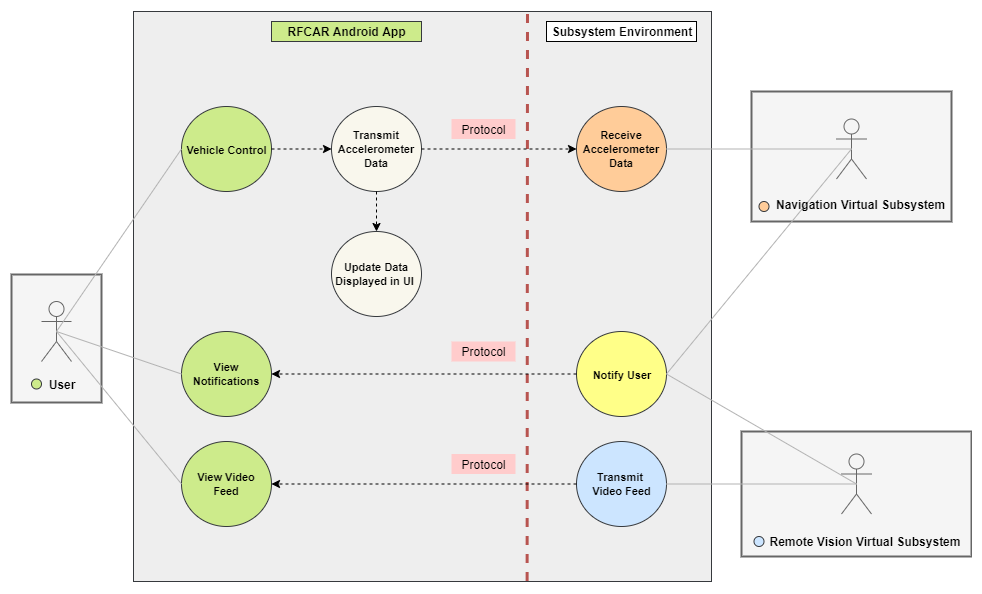
\includegraphics[width=0.8\textwidth]{img/UseCaseAndroid.png}
\caption{\label{fig:usecase_android}Android app use case diagram.}
\end{figure}
%
\subsection{Object/Static Model}
In this step, the objective was to define the app system´s structure with \gls{uml} class diagrams, concerning its objects, attributes, operations and associations established.  The forementioned diagram is represented in figure \ref{fig:uml-android}.
%
\begin{figure}[!ht]
\centering
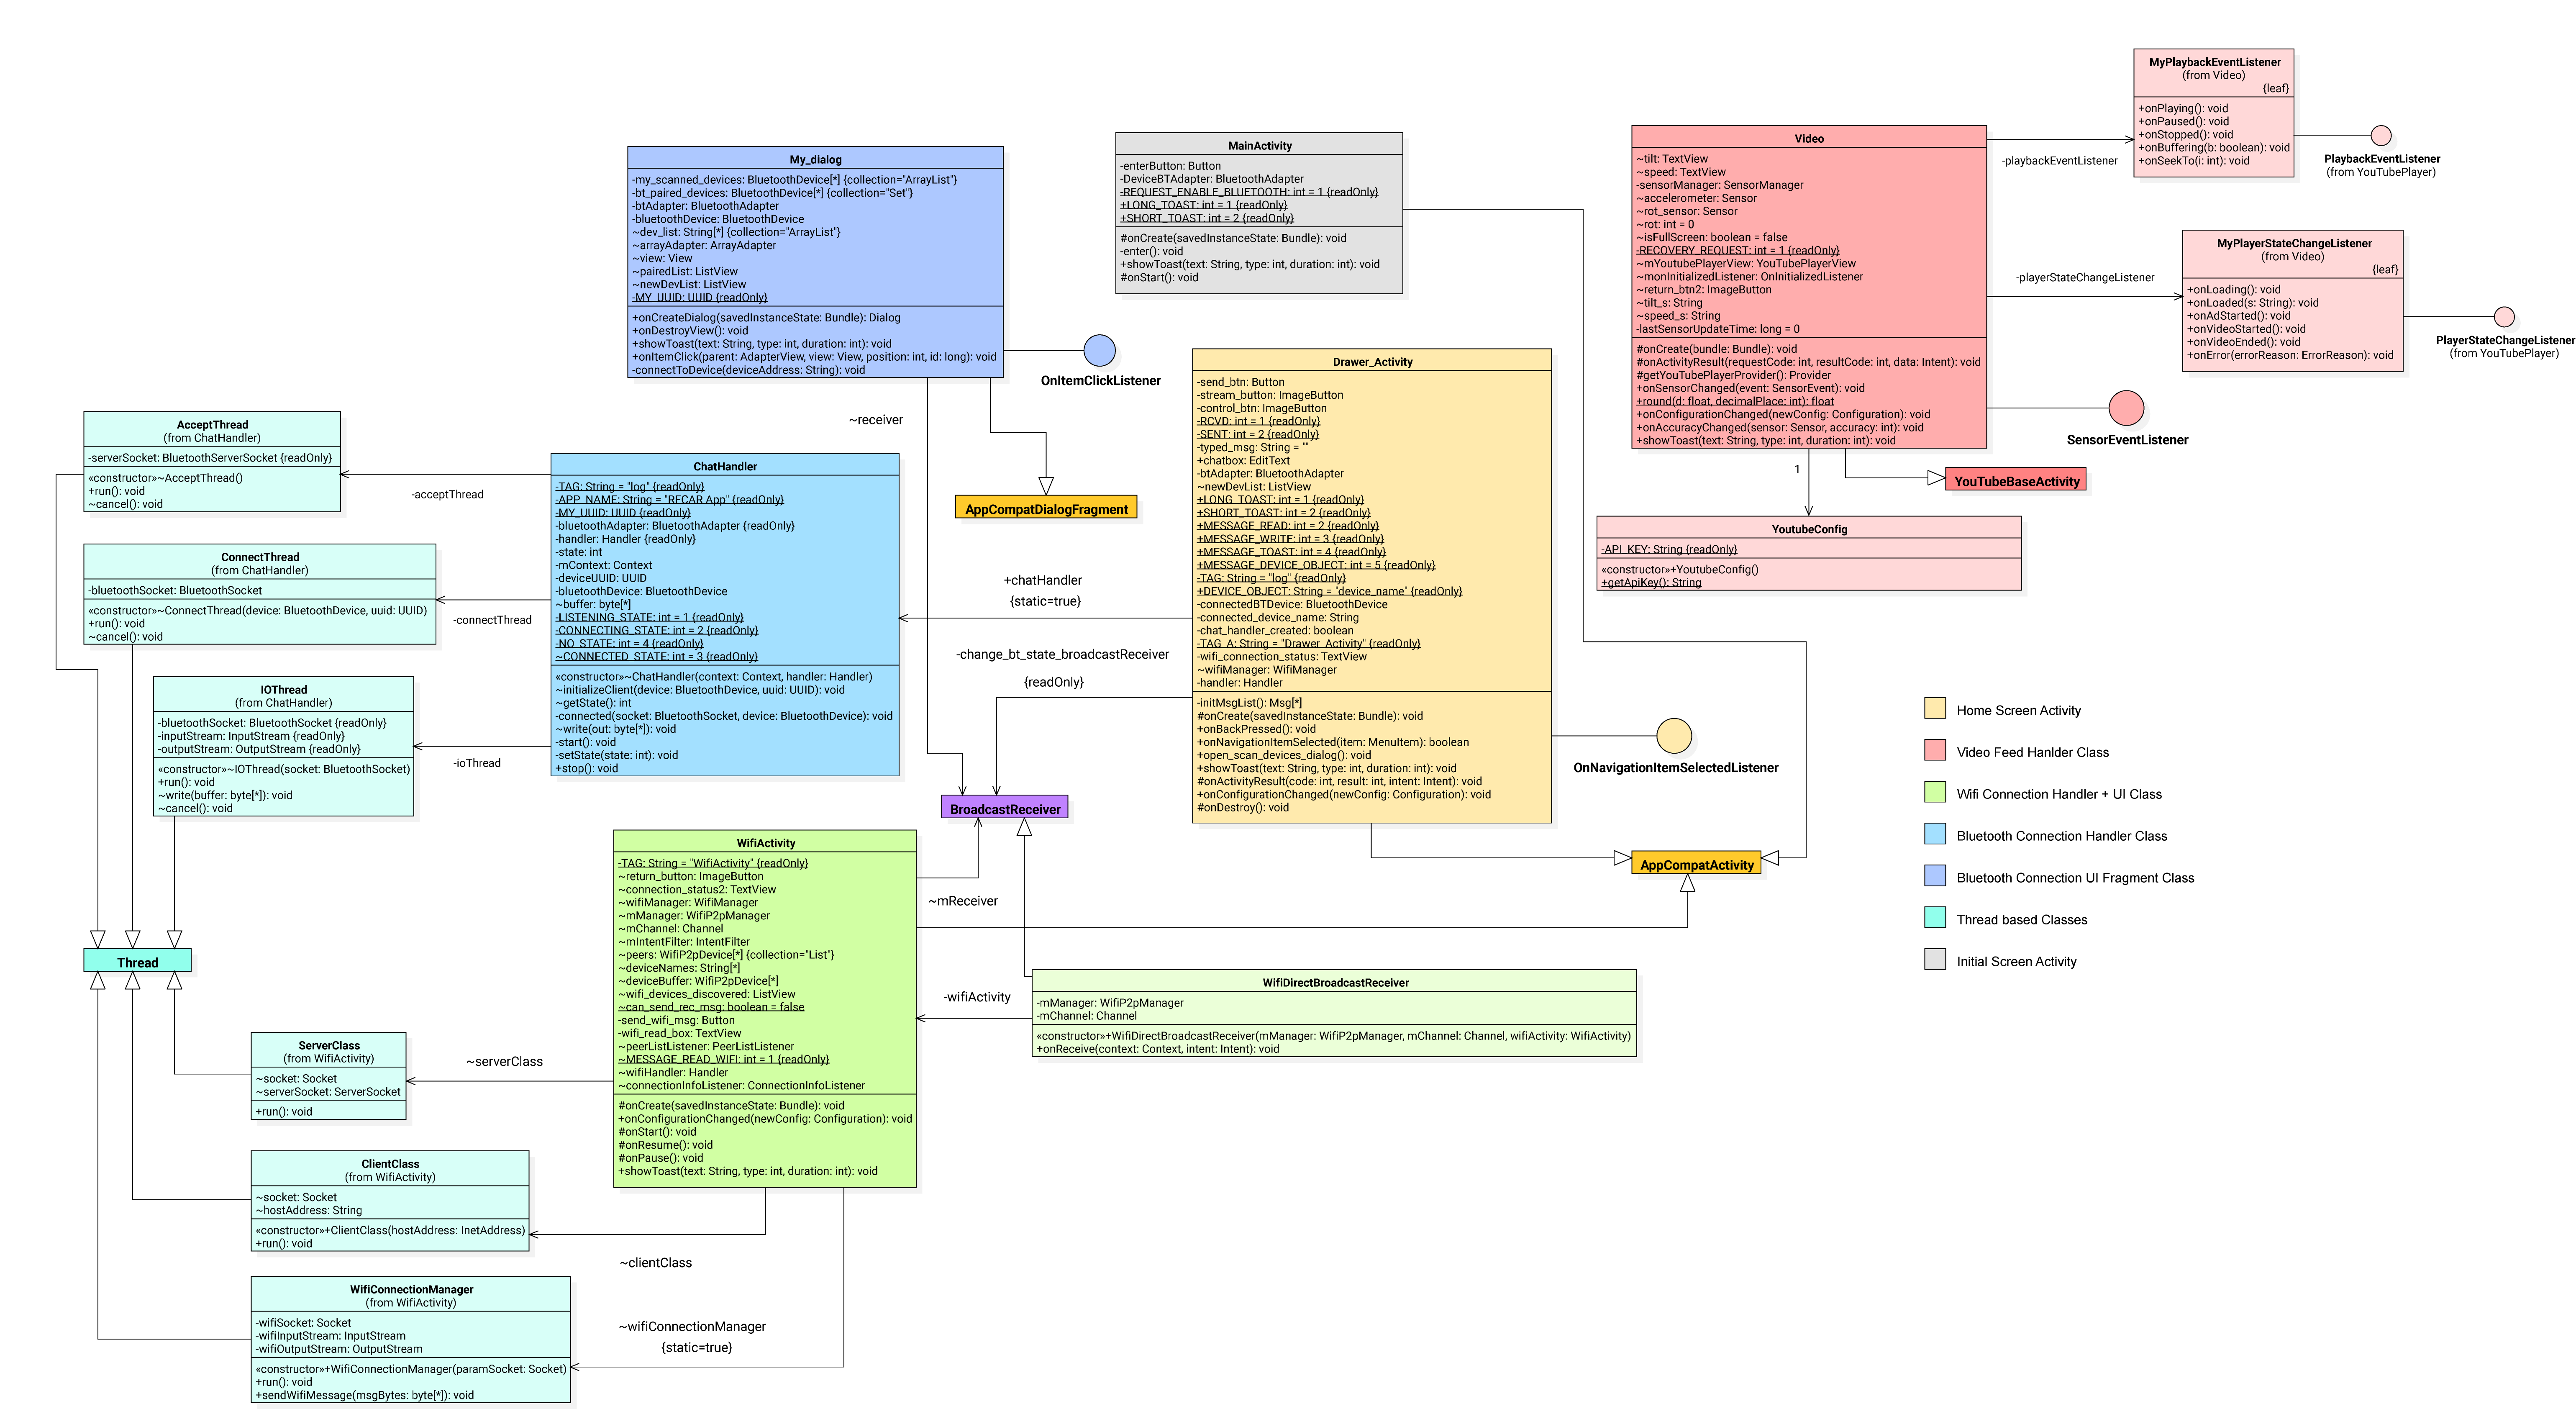
\includegraphics[width=\textwidth]{img/smartphone-static-diagram.png}
\caption{\label{fig:uml-android}Smartphone class diagram}
\end{figure}
%
\subsection{Dynamic Model}
For the dynamic model, were devised multiple state-machine diagrams to describe the internal behaviour of the application. 
%
Figure \ref{fig:overall_system_diagram} illustrates the overall application behaviour. One can observe that all the intended features are meant to run in parallel, that will surely affect the system implementation in terms of concurrency (section \ref{sec:concurrency}) and thread management.
%
Initially, the system loads the \gls{ui} and waits for all connections to be established before moving to the next state.
%
While the feature for vehicle control is running (figure \ref{fig:vehicle_control_diagram}) it retrieves the accelerometer data, sends the data to the \gls{nvs} and displays it on the screen.
%
Additionally, the feature that allows the user to see the video feed transmitted by the \gls{rvvs} in figure \ref{fig:video_feed_diagram} also displays it on the app screen. When this Wifi/GPRS connection is suspended by any means, it should exist an immediate reconnection to the \gls{rvvs}.
%
The notifications presented to the user should indicate the current state of the system, which means displaying informative messages, like successful connections but also alert messages like the ones displayed in figure \ref{fig:notification_diagram}.
%
\begin{figure}[!ht]
\centering
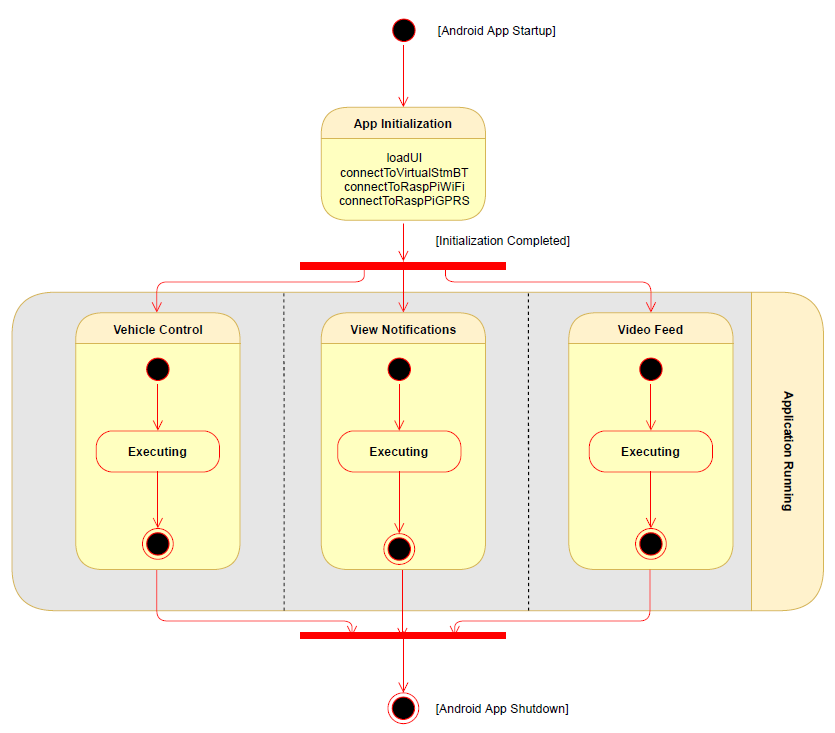
\includegraphics[width=0.7\textwidth]{img/overall_system_sm.png}
\caption{\label{fig:overall_system_diagram}Overall system behaviour diagram.}
\end{figure}
%
\begin{figure}[!ht]
\centering
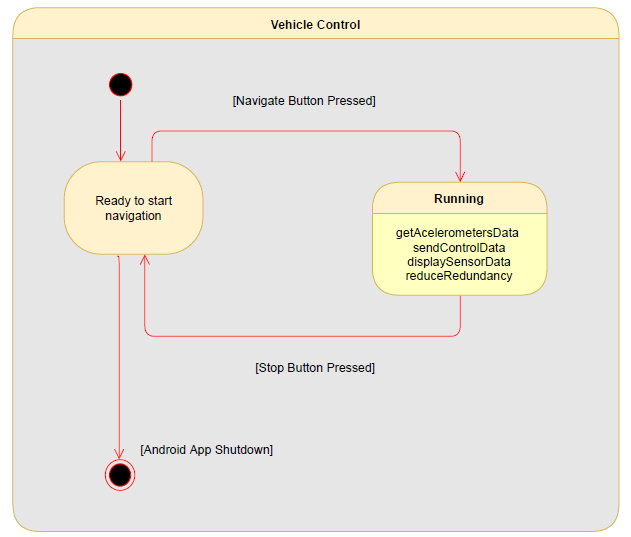
\includegraphics[width=0.7\textwidth]{img/vehicle_control_sm.png}
\caption{\label{fig:vehicle_control_diagram}Vehicle control feature diagram.}
\end{figure}
%
\begin{figure}[!ht]
\centering
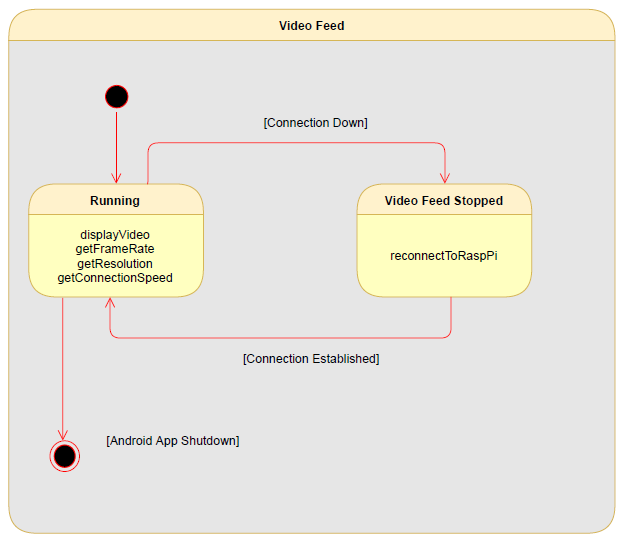
\includegraphics[width=0.7\textwidth]{img/video_feed_sm.png}
\caption{\label{fig:video_feed_diagram}Video feed feature diagram.}
\end{figure}
%
\begin{figure}[!ht]
\centering
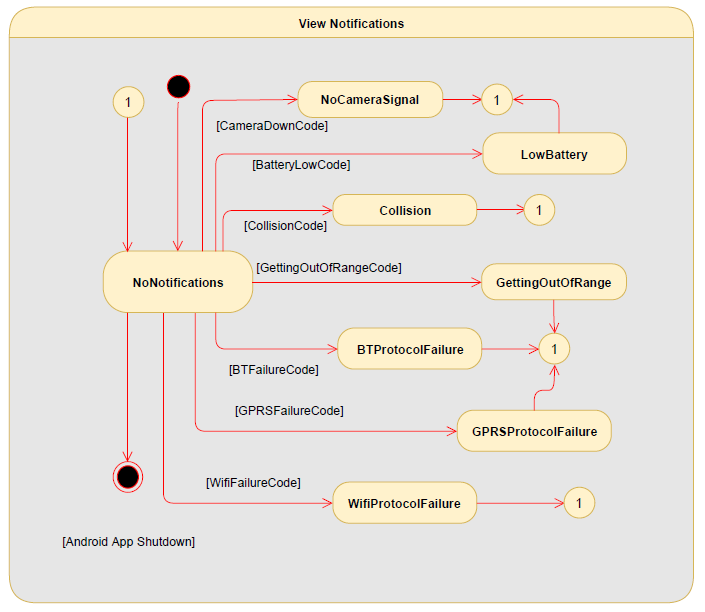
\includegraphics[width=0.7\textwidth]{img/notification_sm.png}
\caption{\label{fig:notification_diagram}Notification feature diagram.}
\end{figure}
%
%
%%% Local Variables:
%%% mode: latex
%%% TeX-master: "../../../dissertation"
%%% End:
